\documentclass{article}
\usepackage{graphicx} % Required for inserting images
\usepackage[utf8]{inputenc} % Per caratteri accentati
\usepackage[T1]{fontenc}    % Per una corretta codifica dei font
\usepackage[italian]{babel} % Per sillabazione in italiano
\usepackage{float}
\usepackage{hyperref}
\usepackage{listings}
\usepackage{color}
\usepackage{amssymb}
\usepackage{amsmath}
\usepackage{multicol}

%VALORI SISTEMABILI
\usepackage[a4paper, top= 1 cm, bottom= 1.5 cm, left= 2 cm, right= 2 cm]{geometry}

\title{Algoritmi e strutture dati}
\author{Francesco Lanzarini}
\date{ }

\begin{document}

\maketitle

\section{Notazione asintotica}
Non ci interessiamo direttamente al tempo esatto di calcolo dell'algoritmo ma la crescita del tempo richiesto rispetto alla crescita dell'input. 
Questa notazione permette di confrontare rapidamente tra loro algoritmi differenti che risolvono lo stesso problema, indipendentemente dall'hardaware.
\subsection{Definizioni e notazioni matematiche}
\paragraph{Funzione di costo}
Associa ad ogni input n la quantità di calcolo necessaria a terminare il calcolo, tutti i numeri sono naturali quindi un numero di bit non negativo e non frazionario ma il codomionio delle funzioni è $\mathbb{R}^+$.
Una volta trovata la funzione di costo ne si sstudia l'andamento asintotico per capirne il \textbf{tasso di crescita}.
\paragraph{O-grande}
Data una funzione $g(n)$ l'insieme delle funzioni $O-grande$ è composto da tutte quelle funzioni con un ordine di crescita inferiorie di $g(n)$; $g(n)$ è dunque il \textbf{limite asintotico superiore}.
\paragraph{$\Omega$-grande}
Data sempre $g(n)$ con $\Omega-grande$ si indica l'insieme delle funzioni con ordine di crescita maggiore o uguale di $g(x)$; $g(x)$ e' dunque il \textbf{limite di crescita inferiore}.
\paragraph{$\Theta$}
Data sempre $g(n)$ si indica con $\Theta$ l'insieme di funzioni che hanno lo stesso ordine di crescita di $g(n)$, 
in altre parole $f(n) = \Theta(g(n)) \iff f(n) = O(g(n)) \land f(n) = \Omega(g(n))$
\paragraph{o-piccolo} La stessa definizione data in analisi ma più specifica essendo in questo caso applicata alle funzioni di costo.
\paragraph{$\omega$-piccolo} Ovvero l'insieme di funzioni che dominano asintoticamente $g(n)$
\paragraph{Complessità computazionale di un algoritmo} Un algoritmo A ha complessità computazionale $O(f (n))$ rispetto ad una certa risorsa di calcolo se la quantità di risorse necessaria per eseguire A su un qualsiasi input di dimensione n è $O(f (n))$.
\paragraph{Complessità computazionale di un problema} Un problema P ha complessità computazionale $O(f (n))$ rispetto ad una certa risorsa di calcolo se il migliore algoritmo che risolve P ha costo computazionale $O(f (n))$ rispetto a tale risorsa di calcolo. 
E' molto più complicata da calcolare rispetto a quella di un algoritmo.
\subsection{Scopo di queste definizioni}
L'ordine di crescita asintotico può essere confrontato attraverso le notazioni di limite, se il limite all'inifnito tra $f(n)$ e $g(n)$ esiste si presentano 3 casistiche:
\begin{itemize}
    \item $\displaystyle \lim_{n \to \infty} \frac{f(n)}{g(n)} = 0$ allora $f(n) =o(g(n)) \Rightarrow f(n) = O(g(n))$
    \item $\displaystyle \lim_{n \to \infty} \frac{f(n)}{g(n)} = \infty$ allora $f(n) =\omega(g(n)) \Rightarrow f(n) = \Omega(g(n))$
    \item $\displaystyle \lim_{n \to \infty} \frac{f(n)}{g(n)} = k >0$ allora $f(n) =\Theta(g(n))$
    
\end{itemize}
Oppure si può utilizzare un'interpretazione intuitiva delle seguenti definizioni:
\begin{figure}[H]
    \centering
    \includegraphics[width=0.4\linewidth]{intuitive notation.png}
    \caption{Interpretazione intuitiva delle definizioni}
\label{fig:intuitive_notation}
\end{figure}


\subsection{Analisi degli algoritmi} 
Solitamente si analizzano 3 aspetti dell'algoritmo:
\begin{itemize}
    \item \textbf{Caso ottimo}: ovvero la complessità computazionale in condizioni ottimali.
    \item \textbf{Caso pessimo}: ovvero la complessità computazionale in condizioni sfavorevoli.
    \item \textbf{Caso medio}: ovvero la complessità computazionale media sul possibile input.
\end{itemize}
Solitamente quando si sviluppa un algoritmo ci si interessa principalmente al caso \textbf{medio/pessimo} 

\subsection{Analisi Ammortizzata}
Serve in caso di algoritmi molto complicati  ed è un metodo per valutare il costo medio di una sequenza di operazioni a differenza di quella degli algoritmi che calcola su singola operazione. Ci sono due metodi principali per fare questo tipo di analisi:
\begin{itemize}
    \item \textbf{Metodo dell'aggregazioni}: si determina un limite superiore al costo totale si una sequenza di n operazioni e dividiamo per n.
    \item \textbf{Metodo degli accantonamenti}: si immagina che ci sia un budget per ogni singola operazione e si accantona il 'resto' che viene usato nel caso il budget non basti per alcune operazioni. Per capire se la stima del budget è corretta alla fine si avrà un surplus positivo, in caso esso sia negativo allora bisogna stimare un budget più alto.
\end{itemize}

\subsection{Equazioni di ricorrenza}
Esprimono il valore di una funzione in termini dei valori su input più piccoli, ci sono due metodi per risolvere le equazioni di ricorrenza:
\begin{itemize}
    \item \textbf{Metodo dell'iterazione}: è un approccio di tipo \textit{brute force} che consiste nell'eseguire iterativamente l'algoritmo in analisi per dedurre il patter e modellizzarlo matematicamente. 
    A questo punto con il caso base si trova il valore dell'icognita $i$ e la si sostituisce nella modellizzazione in modo tale da trovare il costo computazionale dell'algoritmo.
    \item \textbf{Master Theorem}: funziona con equazioni di ricorrenza nella forma $T(n) = aT(n/b) +cn^\beta$ e quindi non puo' essere applicato a tutte le equazioni di ricorrenza (tipo quella di Fibonacci che chiama 2 volte se stessa). Il teorema dice che calcolando $\alpha = log_b(a) = \frac{log(a)}{log(b)}$ ci possono essere 3 casi:
    \begin{enumerate}
        \item Se $\alpha > \beta$ allora $T(n) = \Theta(n^\alpha)$
        \item Se $\alpha = \beta$ allora $T(n) = \Theta(n^\alpha log(n))$
        \item Se $\alpha < \beta$ allora $T(n) = \Theta(n^\beta)$
    \end{enumerate}
    
\end{itemize}

\section{Problema dell'ordinamento}
Sono degli algoritmi che dato in input un array di numeri lo ordinano in modo crescente o decrescente.
Ci sono due proprietà fondamentali di questi algoritmi: \begin{enumerate}
    \item \textbf{In place}: l'algoritmo riordina gli elementi nell'array in input e non ne usa di aggiuntivi
    \item \textbf{Stabile}: valori con la stessa \textbf{chiave} (valore associato all'elemento che è sempre confrontabile con altri elementi) appaiono nell'array ordinato nello stesso ordine di partenza.

\end{enumerate}
\subsection{Algoritmi incrementali}
Sono algoritmi più semplici che costruiscono l'ordinamento dell'array un elemento alla volta, allo stesso tempo però sono anche i meno efficienti
\subsubsection{Selection Sort}
Partendo da un elemento lo scambia con l'elemento minimo presente nel resto dell'array; questa operazione la si ripete per ogni elemento (tranne l'ultimo) andando sempre ad avere a sinistra dell'elmento in analisi un array ordinato.
A causa dell'implementazione degli array la funzione di swap necessita di ulteriore memoria rendendo l'algoritmo $non-stabile$.

\begin{figure} [H]
    \centering
    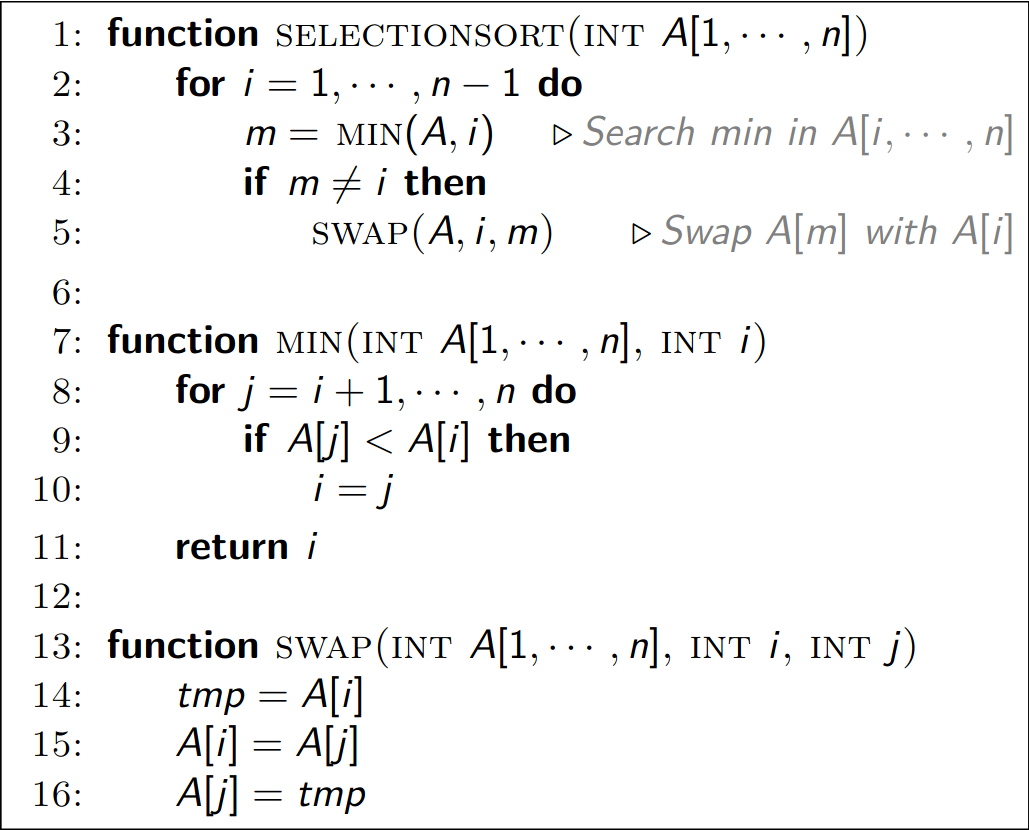
\includegraphics[width=0.5\linewidth]{Selection sort.png}
    \caption{Possibile implementazione del Selection Sort}
    \label{fig:Selectionsort}
\end{figure}

La ricerca del minimo richiede di analizzare tutti gli elementi da $i + 1$ a $n$ ($\Theta(n)$), questa operazione va pero' ripetuta $\Theta(n)$ volte 
portando la complessità computazionale di questo algoritmo a $\Theta(n^2)$.
\subsubsection{Isertion Sort}
Partendo dal secondo elemento e andando verso l'ultimo si inserisce il valore nella parte di array a sinistra nell'ordine giusto scambiandolo con tutti i valori maggiori di esso. 
Per come vengono eseguiti i confronti l'algoritmo è stabile.
\begin{figure}[H]
    \centering
    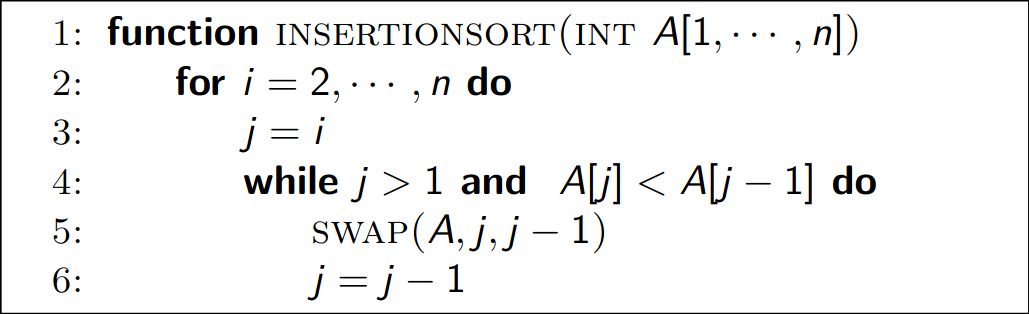
\includegraphics[width=0.5\linewidth]{Insertion sort.png}
    \caption{Possibile implementazione dell'Insertion sort}
    \label{fig:insertionsort}
\end{figure}
Nel caso ottimo il for viene eseguito $n$ volte e basta quindi $\Theta(n)$; nei casi medio e pessimo invece avrà un costo pari a $\Theta(n^2)$.

\subsection{Divide et impera}
Viene dalla tecnica romana e consiste nel dividere il problema in problemi più semplici (\textit{Divide}) che poi vengono risolti in maniera facile (\textit{Conquer}) e poi le soluzioni vengono fuse per risolvere il problema generale.
\subsubsection{MergeSort}
Consiste nello dividere ricorsivamente a metà l'array per poi oridnare i sotto-array che diventano sempre piu' grandi ma allo stesso tempo ogni meta' e' ordinata; questo algorimto può essere implementato in modo stabile.
E' pero' molto complicato implementare questo algoritmo in modo tale che sia anche in-place.

\begin{figure}[H]
    \centering
    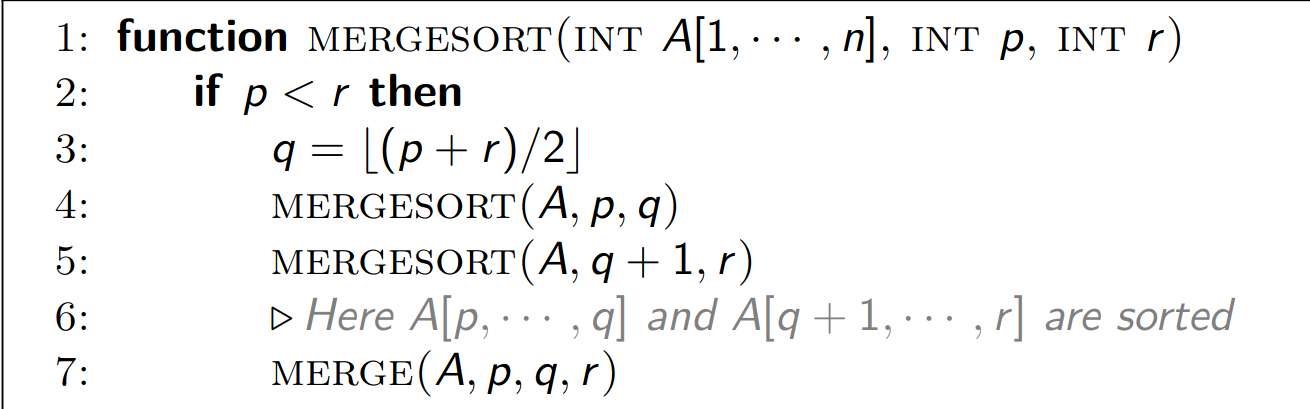
\includegraphics[width=0.65\linewidth]{Mergesortfirst.png}
    \caption{Esempio di implmentazione del MergeSort}
    \label{fig:MergSortfs}
\end{figure}


\begin{figure}[H]
    \centering
    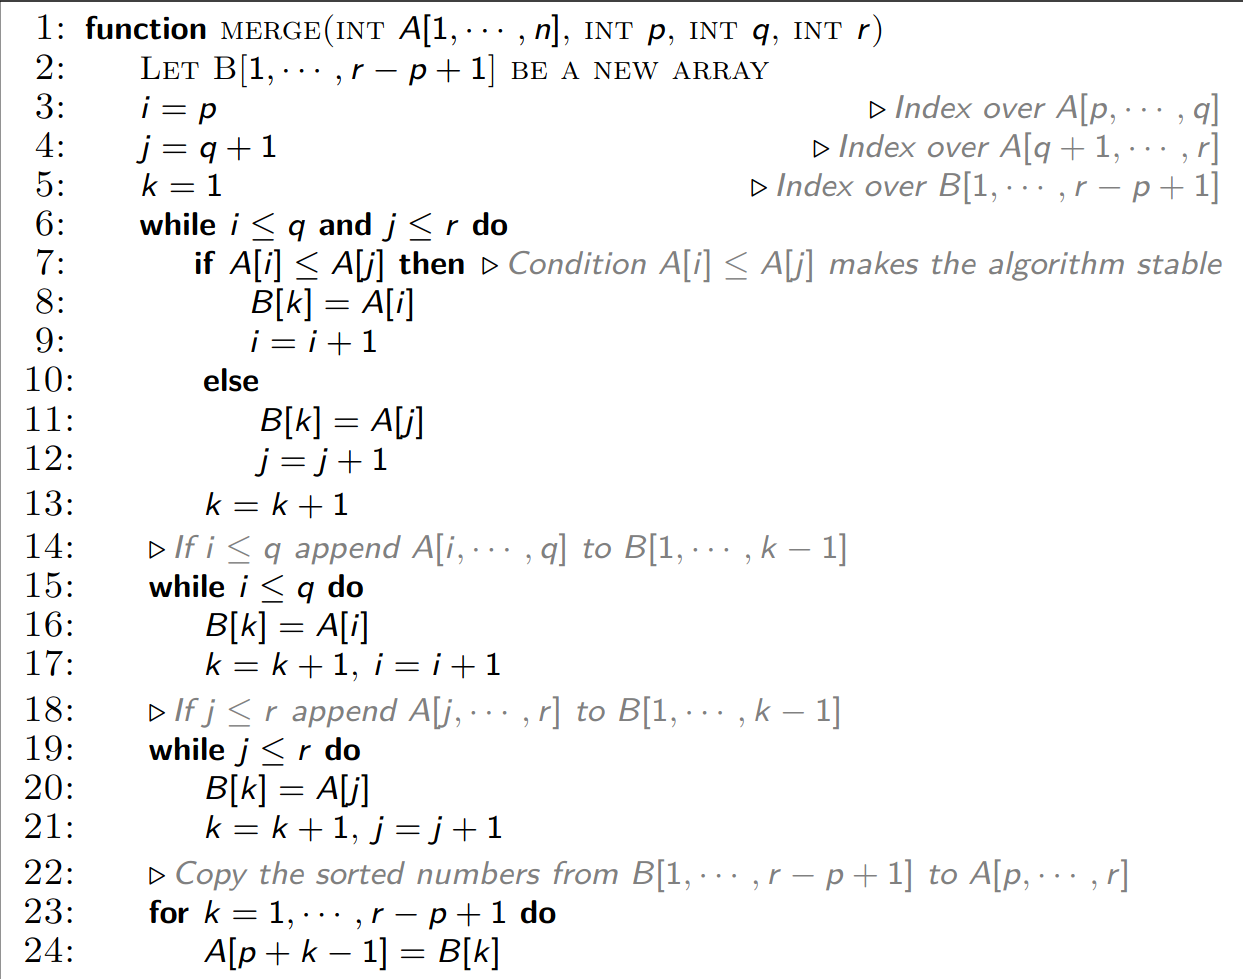
\includegraphics[width=0.65\linewidth]{Merge Sort.png}
    \caption{Esempio di implmentazione della funzione Merge}
    \label{fig:MergSort}
\end{figure}
Questo algoritmo ha complessità $\Theta(nlog(n))$
\subsubsection{QuickSort}
Si sceglie all'interno dell'array un valore detto \textit{pivot} e si riordina l'array in modo tale che tutti i numeri più grandi siano nella parte destra dell'array e tutti i più piccoli sono a sinistra; a livello pratico si ha un contatore che tiene traccia dell'indice dell'ultimo elemento che deve stare a sdinistra del pivot e quando se ne incontra un altro si scambia con quello successivo.
A questo punto si chiama ricorsivamente l'algoritmo nei due sotto array escluso il pivot per riordinare l'array.
Nel caso ottimo il costo è $\Theta(nlog(n))$, nel caso pessimo $\Theta(n^2)$ mentre nel caso medio è $O(nlog(n))$. 
La complessità dipende molto da quale numero si scelga come \textit{pivot} perche' la piu' sono bilanciati i due sotto array piu' e' efficiente l'algoritmo, quindi un'implementazione che sceglie il pivot in maniera furba può rendere l'algoritmo estramamente rapido. 
Nel caso studito si sceglie un numero a caso perche' rende molto improbabile ricadere nel caso pessimo o sfavorevole.
\subsubsection{DualPivot Quicksort}
Crea delle partizioni rispetto a due \textit{pivot} e rende quindi meno probabile ricadere nel caso pessimo ma è anche abbastanza ibrido come algoritmo perchè a seconda delle situazioni può chiamare diversi algoritmi che lo rendono, in generale, molto efficiente; in media ha complessità $O(nlog(n))$.
\subsubsection{Tim Sort}
E' il più recente degli algoritmi che inizialmente fu introdotto in Python e si basa sull'idea che in un array ci siano già delle sottosequenze ordinate e da li usa il merge o insertion per sistemare le sequenze tra di loro. Come complessità ha costo, nei casi medio e pessimo, pari a $O(nlog(n))$ mentre nel caso ottimo $O(n)$.
\subsection{Algoritmi di ordinamento in tempo lineare}
Sono algoritmi che possono essere usati in alcune condizioni speciali perche' un qualsiasi algoritmo di ordinamento basato sulla comparazione di valori non puo' avere un'efficienza migliore fi $\Theta(nlog(n))$ nel caso pessimo.

\subsubsection{Counting Sort}
Questo algoritmo può essere usato solo per ordinare interi all'interno di un intervallo $[a,b]$, esso usa un array d'appoggio di grandezza $k =b-a+1$ per contare quante volte un valore sta nell'array di partenza, riordina l'array senza doppione e riempio l'array di partenza con i numeri in modo ordinato.
\begin{figure}[H]
    \centering
    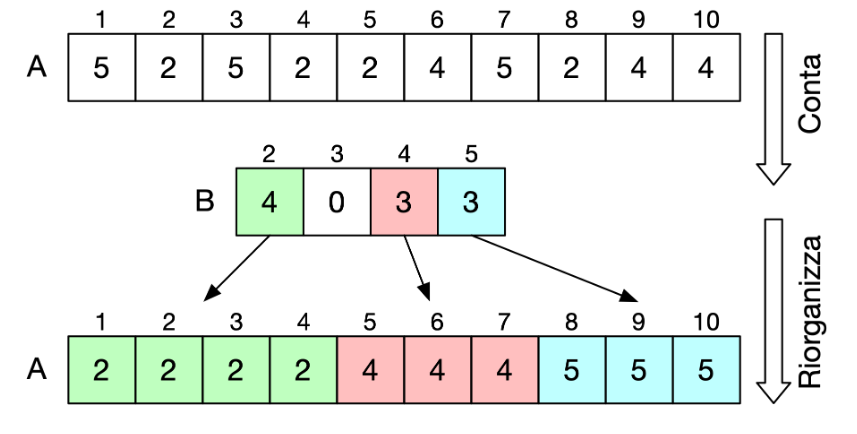
\includegraphics[width=0.5\linewidth]{CountingaSortexample.png}
    \caption{Esempio del funzionamento del CountingSort}
    \label{fig:ExCountingSort}
\end{figure}

\begin{figure}[H]
    \centering
    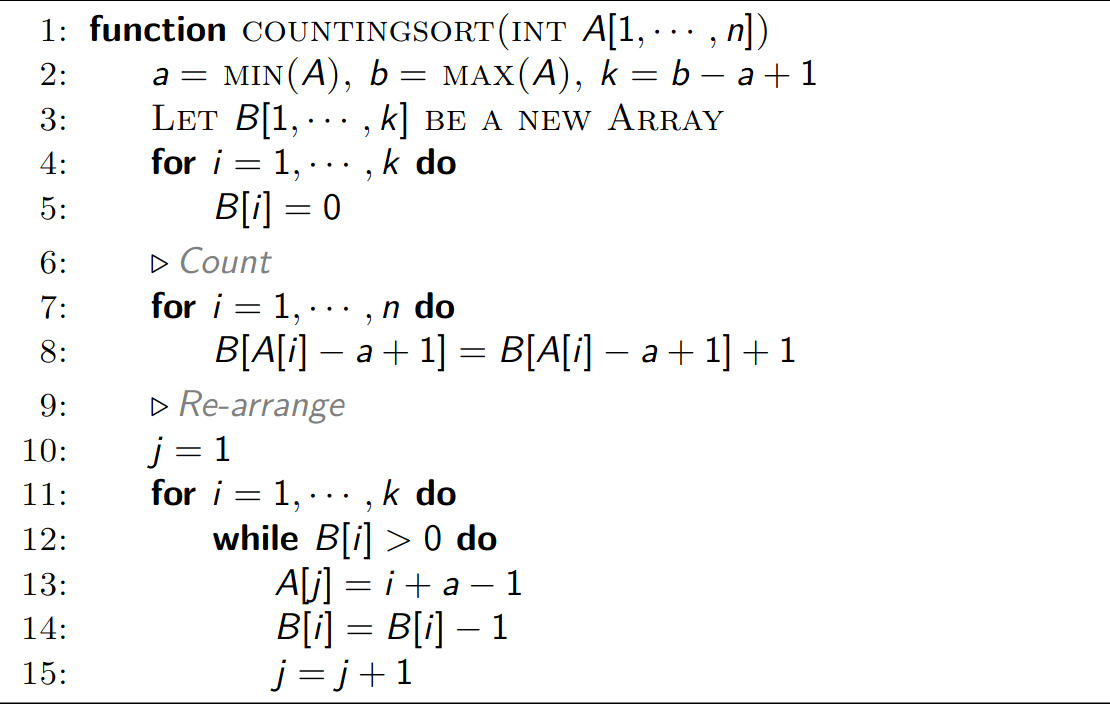
\includegraphics[width=0.5\linewidth]{CountingSort.png}
    \caption{Possibile implementazione CountingSort}
    \label{fig:CountingSort}
\end{figure}

Il costo di questo algoritmo è $\Theta(n+k)$ perchè se k è molto più grande di n o viceversa non è per nulla conveniente.
Per rendere l'algoritmo stabile basta, una volta riempito l'array d'appoggio che conta gli elementi identici, bisogna eseguire le seguenti operazioni:
\begin {enumerate}{
    \item Ricodificare l'array d'appoggio per ottenere l'ultima posizione del dato elemento nell'array finale. Per farlo basta usare la formula:
    \begin{verbatim}
        V[j] = V[j-1] + V[j];
    \end{verbatim}
    \item Riempire l'array finale partendo dall'ultimo elemento dell'array iniziale e metterlo nella posizione codificata dall'array d'appoggio:
    \begin{verbatim}
        A[n]; //given array
        B[a, ..., b]; //support array alredy refactored
        C[n]; //final array
        for (int i = n-1; i >= 0: i--){
            C[B[A[i]]] = A[i];
            B[A[i]]--;
        }
    \end{verbatim}

}
\end{enumerate}
\subsubsection{RadixSort}
Questo algoritmo usa il counting sort come sotto-procedura infatti il RadixSort considera tutti gli interi con lo stesso numero di cifre 
e li riordina rispetto alla cifra meno significativa (attraverso il CountingSort), poi rispetto alla penultima e così via fino a quella più significativa. 
Il costo di questo algoritmo nel caso in cui \textbf{CountingSort} sia stabile (se no non funziona) è di $\Theta(d(n+k))$ con:
\begin{itemize}
    \item $d$ il numero massimo di cifre di una chiave
    \item $k$ è il numero di possibili valori per una cifra
\end{itemize}

\subsection{Riassunto costi degli algoritmi visti}
\begin{figure}[H]
    \centering
    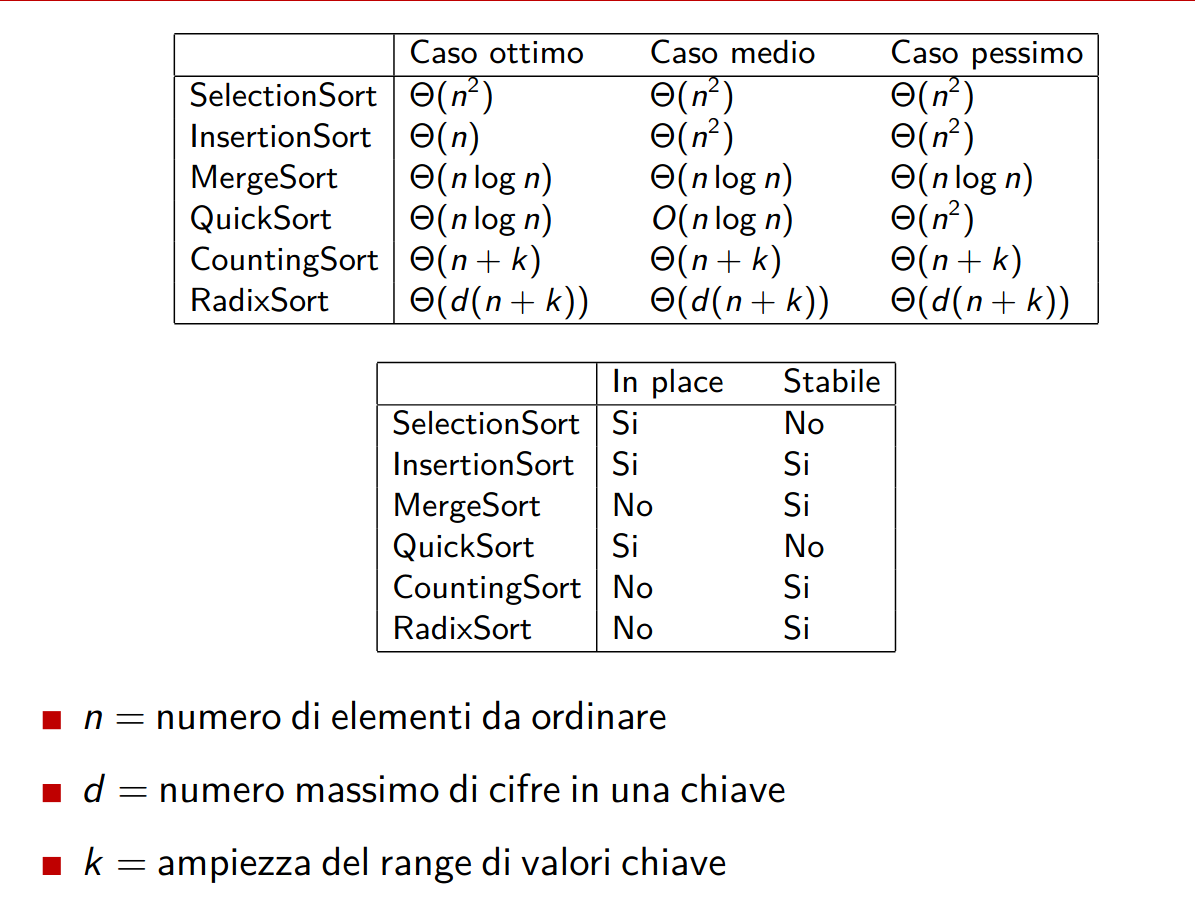
\includegraphics[width=0.65\linewidth]{SummarySort.png}
    \caption{Tabella riassuntiva dei costi degli algoritmi di ordinamento esaminati}
    \label{fig:SummarySorting}
\end{figure}
\section{Strutture di dati elementari}
Descrivono come sono \textbf{logicamente organizzati} i dati e ne definisce le \textbf{operazioni} per cui non si hanno informazioni riguardo a \textbf{quali} dati sono memorizzati.
Ci sono due parti principali delle strutture dati:
\begin{itemize}
    \item \textbf{Prototipo} \begin{itemize}
        \item Descrive possibili valori e operazioni
        \item Nasconde i dettagli implementativi
        \item Permette di implementare la struttura
        \item Permette di capire come usare la struttura
    \end{itemize}
    \item \textbf{Implementazione} \begin{itemize}
        \item Realizzazione di una struttura dati in uno specifico linguaggio di programmazione
        \item Non visibile all'utente
        \item Può influire sui tempi di esecuzione
    \end{itemize}
\end{itemize}

\subsection{Liste}
Struttura di dati in cui tutti gli elementi sono organizzati in modo sequenziale e deve supportare almeno le operazioni di \textbf{ricerca, inserimento e rimozione}. 
Esse si possono implementare sia con strutture primitive ovvero degli \textit{array} che hanno il vantaggio di avere un tempo di accesso lineare ma hanno una grandezza fissa dipendete dallo spazio di memoria contigua libera, 
oppure attraverso \textit{linked list} che non dipendono dalla quantità di memoria contigua libera ma hanno un tempo di accesso agli elementi dipendete dalla lunghezza della lista.
\subsubsection{Linked List semplice}
Ogni nodo punta al successivo quindi la si puo' scorrere in un solo verso, le operazioni hanno i seguenti costi: \begin{itemize}
    \item \textbf{Search}: e' implementata attraverso una semplice ricerca lineare per cui ha costi:
    \begin{itemize}
        \item Ottimo: $O(1)$
        \item Medio: $\Theta (n)$
        \item Pessimo: $\Theta(n)$
    \end{itemize}
    \item \textbf{Insert}: inserimento in testa alla coda:
    \begin{itemize}
        \item Ottimo: $O(1)$
        \item Medio: $O(1)$
        \item Pessimo: $O(1)$
        \end{itemize}
    \item \textbf{Append}: inserimento in coda, per cui e' necessario scorrere tutta la lista:
    \begin{itemize}
        \item Ottimo: $\Theta (n)$
        \item Medio: $\Theta (n)$
        \item Pessimo: $\Theta (n)$
        \end{itemize}
    \item \textbf{Delete}: simile all'operazione di search ma elimina l'elemento: 
    \begin{itemize}
        \item Ottimo: $O(1)$
        \item Medio: $\Theta (n)$
        \item Pessimo: $\Theta (n)$
        \end{itemize}

\end{itemize}

\subsubsection{Double Linked List}
Sono come le Linked list semplici ma hanno un puntatore al nodo precedente quindi possono essere lette anche al "contrario". Nonostante ciò tutte le operazioni hanno lo stesso costo computazionale delle Linked List normali ma si deve usare più memoria per ogni singolo elemento.

\subsubsection{Linked List circolari}
Sono \textit{Double Linked List} ma con la differenza che l'ultimo e il primo elemento si puntano a vicenda in modo che sia logicamente circolare, 
i costi invariati rispetto alle altre tranne per l'inserimento in coda che è costante.

\subsubsection{Linked List con puntatori a testa e coda}
Come una normale Linked List con la differenza che si ha un puntatore anche per la coda della lista per cui 
costi computazionali rimangono invariati tranne per l'inserimento in coda che è costante.

\subsection{Pila}
La struttura pila supporta due operzioni principali: il \textbf{push} (aggiunta di un elemento) e \textbf{pop} (eliminazione dell'elemento più recente). 
Questa struttura dati si può implementare sia attraverso un array che con una lista. Nel caso di uso di un array \textbf{statico} ci possono essere errori di underflow/overflow ma costi computazionali costanti, mentre con un \textbf{array dinamico} si puo' variare l'array ma avendo un costo medio di $O(n)$ per ognuna delle operazioni.

\subsection{Code}
Questa struttura dati supporta solo due operazioni principali: \textbf{enque} (aggiunta di un elemento in fondo) e \textbf{dequeue} (rimuove l'ultimo elemento della coda); in pratica si tartta di \textit{Linked List} con operazioni limtate.
Questa struttura dati puo' essere efficientemente implementata (ovvero le operazioni hanno costo costante) attraverso \textit{Linked list circolari}, \textit{Linked List semplici} o \textit{array circolari}.

\subsection{Alberi}
Sono strutture dati \textbf{gerarchiche}, a differenza delle precedenti che sono dette \textit{lineari}, definite da:
\begin{itemize}
    \item \textbf{Nodi}
    \item \textbf{Archi} che connetono i nodi
    \item Esiste \textbf{un solo percorso} da un nodo all'altro
\end{itemize}
Un albero puo' essere \textbf{ordinato} sse i figli di ogno nodo sono ordinati (primo, secondo, ...) e \textbf{radicato} ovvero se uno dei suoi nodi puo' essere identificato come radice.

\subsection{Alberi Binari}
Sono alberi in cui ogni nodo ha al massimo 2 figli, dunque, potendo identificare \textit{figlio destro} e \textit{figlio sinistro}, e' per definizione \textbf{ordinato} .
La \textbf{profondita'} di un nodo e' la lunghezza dell'unico percorso che lo collega con la radice, 
questo numero e' identico a quello degli archi che collegano nodo-radice mentre un \textbf{livello} e' l'insieme di tutti i nodi su uno stesso livello. 
Per \textbf{altezza} di un albero si intende la massima profondita' (per convenzione si considera -1 la profondita' di un albero vuoto), mentre il \textbf{grado} di un nodo e' il numero dei suoi figli.
Un albero binario si dice \textbf{completo} sse ogni nodo ha due figli e un albero \textbf{perfetto} e' un albero completo con tutte le foglie alla stessa profondita'.
\paragraph{Proprieta' fondamentale degli alberi} Ogni albero non vuoto ha esattamente $n - 1$ archi, con n il numero di nodi dell'albero.
\subsection{Algoritmi di visita}
Sono algoritmi per visitare tutti i nodi di una struttura dati albero.
\subsubsection{Visita in profondita'}
La ricerca va il piu' in profondita' possibile prima di visitare i nodi nello stesso livello
\begin{itemize}
    \item \textbf{Pre-order}: visita il nodo stesso poi l'albero sinistro e infine quello destro; la sua complessita' e' $\Theta(n).$
    \item \textbf{Post-order}: visita l'albero sinistro poi quello destro e infine il nodo stesso; la sua complessita' e' $\Theta(n).$
    \item \textbf{In-order}: visita l'albero sinistro poi il nodo stesso e infine quello destro; la sua complessita' e' $\Theta(n).$
\end{itemize}
\subsubsection{Visita in ampiezza}
La ricerca viene eseguita livello per livello
\begin{itemize}
    \item \textbf{Visita in ampiezza}: in pratica si fa una coda e ad ogni ciclo si toglie dalla coda il nodo e si mettono in coda i nodi in modo che ci sia una stampa per livello; la complessita' e' sempre $\Theta(n).$
\end{itemize}

\subsection{Come contare tutti i nodi di un albero?}
Inizialmente si potrebbe pensare di implementare un algoritmo con la stessa idea di fondo della visita che al posto di stampare valori conta i nodi ma questo richiederebbe una complessita' pari a $\Theta(n)$, esiste dunque un modo di rendere la complessita' di questa operazione costante aggiungendo un campo ad ogni nodo che permette di memorizzare il numero di nodi sottostanti ad esso. Questo pero' rende piu'dispendiosa una qualsiasi modifica dell'albero.


\subsection{Alberi binari di ricerca (BST)}
Sono alberi radicati con vincoli sull'organizzazione delle chiavi: tutte le chiavi a sinistra di un nodo sono minori di esso mentre tutte quelle a destra sono maggiori;
con questa organizzazione è possibile fare una ricerca binaria su questa struttura dati e le visita \textbf{in-order} permette di stampare in ordine tutti gli elementi dell'albero. 
Le operazioni fondamentali su questa struttura dati sono:
\begin{itemize}
    \item \textbf{Search}: ritorna il nodo con chiave $k$, essa sfrutta la topografia della struttura infatti confrontando il valore cercato con la chiave del singolo nodo si sposta a destra nel caso $k>node.key$, al contrario si sposterà a sinistra. Questa operazione ha un costo nel caso pessimo pari a tutti i nodi (caso albero degenere).
    \item \textbf{Insert}: inserisce un nodo, anche questa operazione sfrutta la topologia della struttura dati ed e' simile alla search, nel caso pessimo, ovvero l'albero degenre, ha una complessita' $\Theta(n)$, mediamente il costo dipende pero' dall'altezza dell'albero.
    \item \textbf{Delete}: rimuove un elemento dalla struttura dati, questa operazione necessita pero' di alcune operazioni di supporto: \begin{itemize}
        \item \textbf{Max}: ritorna il nodo massimo nell'albero ovvero lo percorre scegliendo sempre il figlio destro.
        \item \textbf{Min}: ritorna il nodo minimo nell'albero ovvero lo percorre scegliendo sempre il figlio sinistro.
        \item \textbf{Predecessor}: ritorna il nodo precedente a T in una visista in-order. Per quanto riguarda l'implementazione ci sono due casi distinti: 
        \begin{itemize}
            \item \textbf{Caso 1}: il nodo di cui si vuole trovare il precdecessore ha un figlio sinistro: il nodo predecessore e' il nodo con chiave massima nel sotto-albero sinistro.
                                   Per trovarlo e' necessario usare la funzione max nel sotto-albero sinitro: $pred\ =\ max(T.left)$ 
            \item \textbf{Caso 2}: il nodo di cui si vuole trovare il predecessore non ha un figlio sinistro; il nodo predecessore e' il primo antenato per cui il nodo di cui si sta cercando il predecessore e' nell'sotto-albero destro.
                                   Per trovarlo e' sufficiente ripercorrere l'albero verso l'alto (trmite il campo $parent$) fino a quando $N\_pred = T.left$
        \end{itemize}
        \item \textbf{Successor}: simmetrico a predecessor.
    \end{itemize}
Anche nel caso della rimozione ci sono tre casi da considerare nell'implementazione:
\begin{itemize}
            \item \textbf{Caso 1}: Il nodo da rimuovere e' una foglia, questo caso e' semplice perche' la regolarita' dell'albero non viene intaccata.
            \item \textbf{Caso 2}: Il nodo da rimuovere ha un solo figlio; in questo caso il figlio del nodo da rimuovere diventa il figlio del genitore del nodo da rimuovere.
            \item \textbf{Caso 3}: Il nodo da rimuovere ha 2 figli; in questo caso si copiano i dati del predecessore del nodo da rimuovere nel nodo stesso e si rimuove il nodo di cui sono stati copiati i dati.
        \end{itemize}
    \end{itemize}
A livello implementativo si usano 2 funzioni: la funzione \textbf{delete} che scambia i nodi nel caso 2 e 3 mentre la funzione \textbf{disconnect} che disconnette il nodo cfon controlli per casi particolari.
\subsection{Riassunto}
\begin{figure}[H]
    \centering
    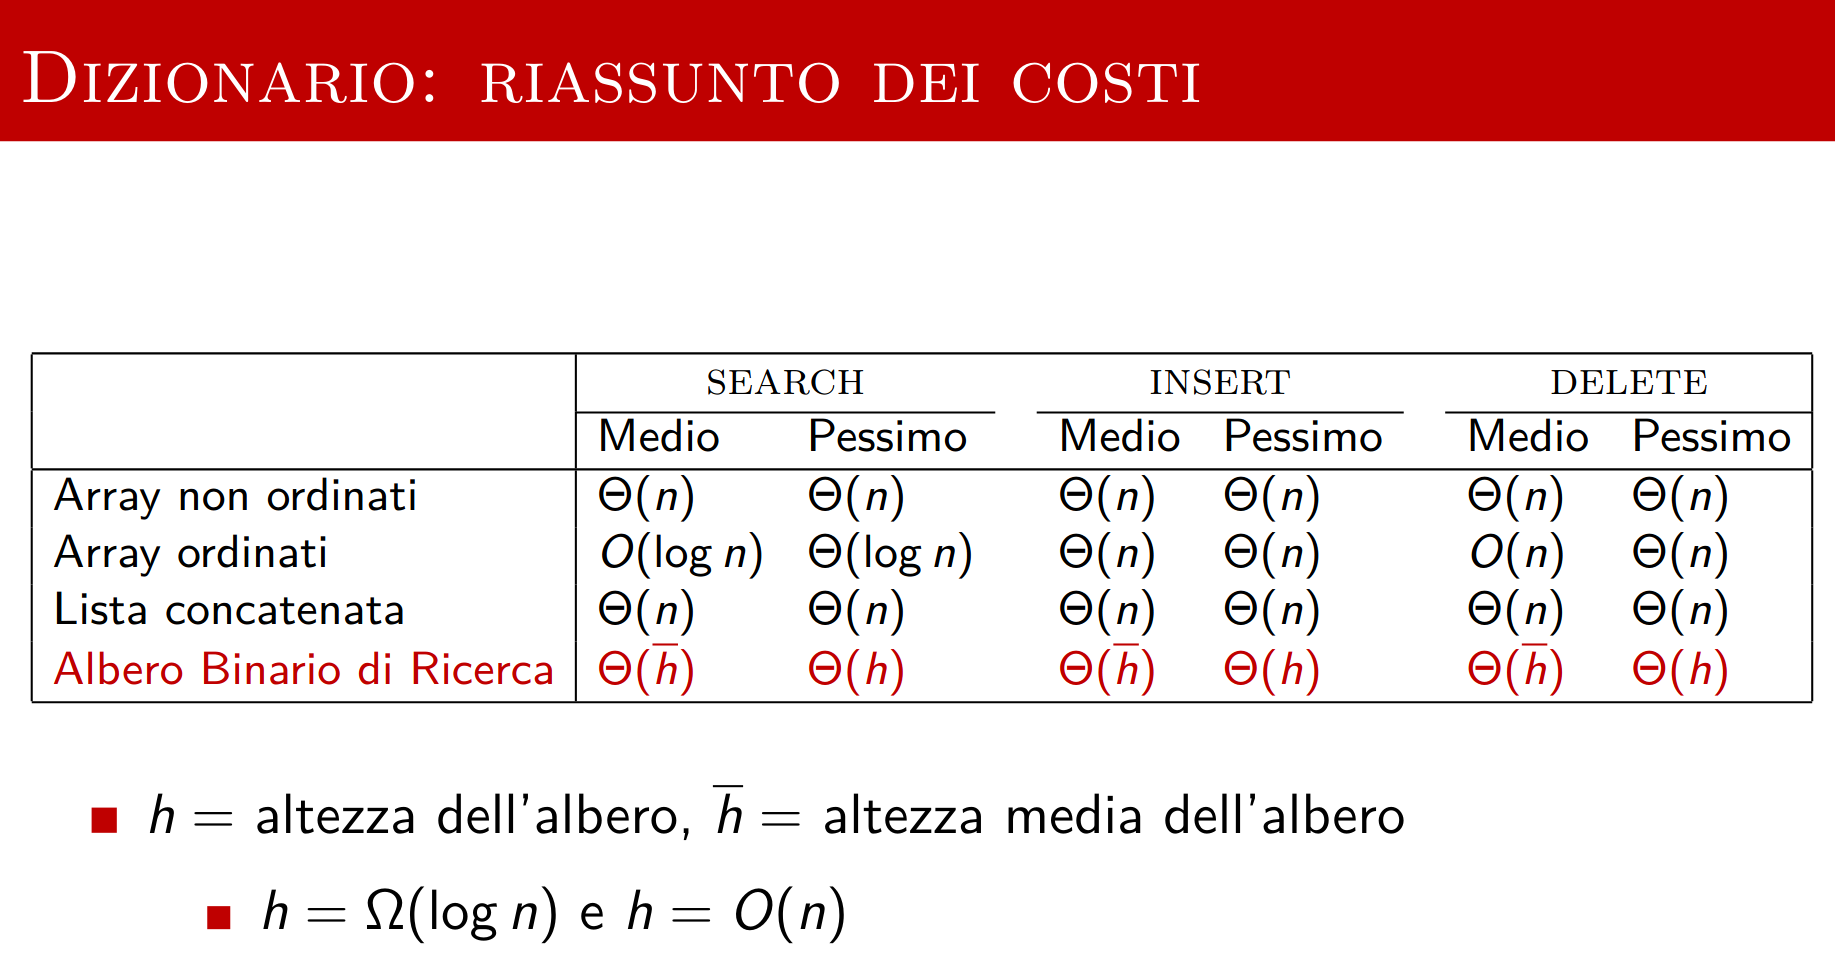
\includegraphics[width=0.5\linewidth]{Riassunto BTS.png}
    \caption{Riassunto costi strutture viste fino a questo punto}
    \label{fig:riassunto_bts}
\end{figure}

\subsection{Alberi AVL}
Prendono il nome dai loro inventori, sostanzialmente sono dei BTS (alberi binari di ricerca) gestiti in maniera tale che siano sempre bilanciati, questo permette di avere un costo delle operazioni nel caso pessimo sempre di $O(log(n))$. 
Per renderelo possibile e' necessario modificare le operazioni di aggiunta e rimozione in modo tale da avere un albero sempre bilanciato.
\subsubsection{Quando posso dire che un albero e' bilanciato?}
Definiamo inizialmente il \textbf{fattore di bilanciamento} (riferito ad un nodo), ovvero la differenza tra l'altezza del suo sotto albero di sinistra con quello di destra: 
\begin{center}
    $\beta (v)=altezza(v.left)-altezza(v.right)$
\end{center}
A questo punto possiamo definire un \textbf{albero bilanciato} in altezza come un albero in cui ogni nodo la differenza di altezza tra i suoi sotto-alberi non e' mai maggiore di uno:
\begin{center}
    $|\beta(v) \leq 1| $
\end{center}

\subsubsection{Operazioni basiche}
\begin{enumerate}
    \item \textbf{Search}: viene eseguita come una normale ricerca su un albero BTS dato che non cambia nessun elemento dell'albero.
    \item \textbf{Update height}: aggiorna l'altezza dell'albero, ogni nodo ha un suo paramentro che contiene l'altezza del sotto albero sottostante
    \item \textbf{Balance factor}: aggiorna il fattore di bilanciamento di un nodo tramite il campo height dei suoi figli.
    \item \textbf{Rotazioni}: esse sono fondamentali per ribilanciarte alberi AVL che, in seguito a modifiche, non sono piu' bilanciati.
    L'operazione di rotazione modifica il fattore di bilanciamento dei soli due nodi coinvolti nell'operaziome.
    A livello implemntativo la \textbf{rotazione a destra} del nodo u consiste nel considerare il suo figlio sinistro (nodo v) e rendere il figlio destro di v il figlio sinistro di u; 
    fatto questo il nodo u diventa il figlio destro di v con opportuni controlli ed aggiustamenti.
    Al contratio, l'operazione di \textbf{rotazione a sinistra} del nodo v consiste nell'individuare il figlio di destra di v (il nodo u) e far diventare sotto-albero destro il soottoalbero sinistro di u;
    fatto cio' il nodo v diventa sotto-alberio sinistro del nodo u con opportuni controlli ed aggiustamenti. 
    \begin{figure}[H]
        \centering
        \includegraphics[width=0.55\linewidth]{rotations.png}
        \caption{Esempio e proprieta' delle rotazioni}
        \label{fig:ratation}
    \end{figure}
    Nel caso dunque che un albero AVL diventi sbilanciato si possono verificare 4 situazioni diverse:
    \begin{figure}[H]
        \centering
        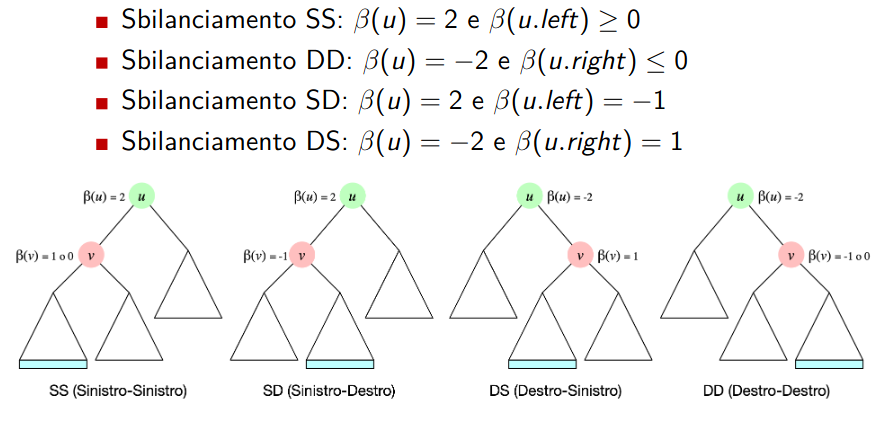
\includegraphics[width=0.75\linewidth]{Rotations_case.png}
        \caption{Casi di sbilanciamento degli alberi}
        \label{fig:caserotation}
    \end{figure}
    A questo punto si illustrano i modi per ribilanciare gli alberi nelle varie situazioni: \begin{itemize}
        \item \textbf{SS}: si esegue una rotazione a destra con perno il nodo con $\beta(n) = 2$.
        \item \textbf{SD}: si esegue una rotazione a destra sul sotto-albero sinistro in modo da avere uno sbilaciamento SS e poi si bilancia come un normale SS.
        \item \textbf{DD}: opposto al caso SS, dunque si opera una rotazione a sinistra con perno il nodo sbilanciato.
        \item \textbf{DS}: si opera una rotazione a destra sul sottoramo destro e poi si risolve come un DD
    \end{itemize}
    \item \textbf{Bilanciamento}: funzione molto semplice perche' si basa sulle funzioni descritte sopra, il suoi unico compito e' verificare il tipo di sbilanciamento e chiamare le funzioni di rotazione su gli opportuni nodi per cui ha costo costante.
    \item \textbf{Insert}: inserisce un nodo come in un normale BST ma alla fine chiama la funzione di bilanciamento dell'albero, al massimo puo' aver sbilanciato al massimo un solo nodo 
    per cui il ciclo che aggiorna il campo height dei nosi soprastanti a quello inserito si ferma o quando si arriva alla radice oppure appena si trova il nodo sbilanciato e lo si sistema.
    Grazie alla topografia di questa struttura dati l'operazione ha costo $\Theta(log(n))$.
    \item \textbf{Delete}: anche in questo caso viene utilizzata la funzione dei BST ma questa procedura puo' comportare lo sbilanciamento di piu' nodi per cui occorre verificare il bilanciamento di ogni singolo nodo di cui si aggiorna il campo height.
\end{enumerate}

\subsubsection{Riassunto}
\begin{figure}[H]
    \centering
    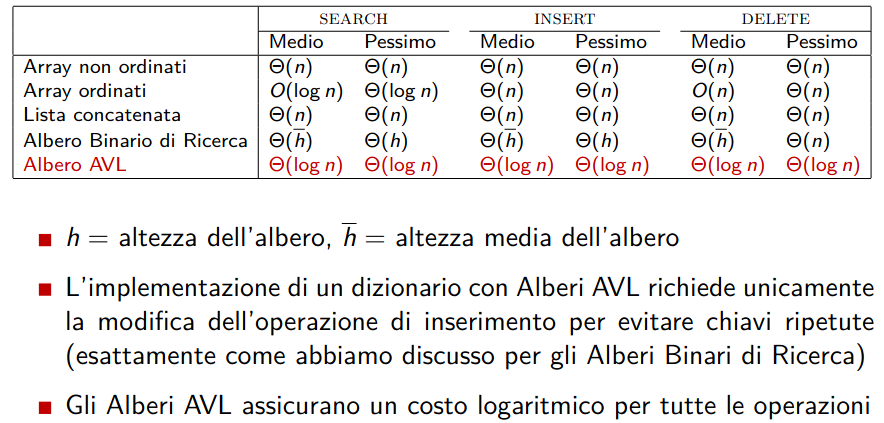
\includegraphics[width=0.75\linewidth]{SummaryAVL.png}
    \caption{Riassunto costi delle operazioni delle strutture visto fino ad ora}
    \label{fig:Summaryavl}
\end{figure}

\section{Tabelle HASH}
L'idea dietro a questa struttra e' quella di replicare l'indicizzazione di un array in una struttura dati dinamica.
In questo modo, sotto le opportune ipotesi, tutte le operazioni di base hanno un costo medio che è costante mentre solo il pessimo ha costo lineare.
Ci sono due principali implementazioni che si usano in casi diversi: le \textbf{tabelle ad indirizzamento diretto} che si usano quando il numero di chiavi effettivamente utilizzate è circa lo stesso numero di tutte le chiavi possibili 
e le \textbf{tabelle HASH} che vengono usate quando il numero di chiavi utilizzate e' molto minore rispetto a quello di chiavi possibili.

\subsection{Tabelle ad indirizzamento diretto}
Sono implementate tramite array dalla dimensione statica, ogni elemento contiene sia una chiave per essere riconosciuta che un campo per il vlore in se. 
In realtà la chiave è la posizione dell'elemento all'interno dell'array (unica struttura dati a indirizzamento diretto), le operazioni basilari come \textit{search, insert e delete} hanno un costo computazionale pari a $O(1)$ ma il vero problema e' la memoria che viene utilizzata: 
se le chiavi realmente utilizzate sono molte meno di quelle disponibili allore c'e' un alto spreco di memoria; stesso discorso nel caso di un insieme universo con molte chiavi che porta ad un'enorme necessità di memoria.
\subsection{Tabelle Hash}
Con le tabelle HASH si cerca una soluzione al problema della memoria attraverso una \textbf{funzione di HASH} $h:U \to [0, ..., m-1]$ 
che partendo dalla chiave del dato da memorizzare è in grado di mappare un indirizzo dell'array. 
Il problema di questa implementazione è l'inevitabile presenza delle \textbf{collisioni} ovvero due chiavi differenti sono mappate nello stesso indirizzo dell'array.

\subsection{Funzione Hash}
Una buona funzione di hash soddisfa la proprieta' di \textbf{uniformita' semplice} ovvero c'e' un equiprobabilita' di generare ogni chiave perche' nel caso ci siano indici che vengono scelti piu' frequentemente come conseguenza si avranno sicuramente maggiori coillisioni. Essendo pero' questo irrealistico ci sono 3 assunzioni che vengono fatte riguardo ad una funzione hash: \begin{enumerate}
    \item Tutte le chiavi sono \textbf{equiprobabili} anche se non e' sempre vero.
    \item La complessita' di calcolo della funzione hash e' $O(1)$ perche' se no costerebbe di piu' calcolare la funzione che cercare l'elemento all'interno dell'array.
    \item Tutte le chiavi sono numeri interi e non negativi.
\end{enumerate}
\subsubsection{Metodo della divisione}
Si restituisce il modulo tra il valore e la lunghezza della tabella, nel caso siano stringhe si convertono i singoli caratteri in valori numerici tramite la rappresentazione binaria. 
Questo metodo è molto efficiente ma dipende in modo molto stretto dalla scelta della lunghezza, infatti se la dimensione dell'array fosse 10 del valore si utilizzerebbe solo l'ultima cifra, mentre se la lunghezza fosse $2^p$ allora di un valore da mappare solo\ i $p$ bit meno significativi nella rappresentazione binaria.

\subsubsection{Metodo delle moltiplicazioni}
Usano la formula $h(k) = \lfloor m(kC-\lfloor kC\rfloor)\rfloor$ con \begin{itemize}
    \item $m$ = numero di slot nell'array
    \item $0 < C < 1$
    \item $\lfloor x\rfloor$ = parte intera di $x$
\end{itemize}
$C$ influenza l'uniformità di $h(k)$ ma il valore di $m$ in questo caso non è critico.

\subsubsection{Metodo della codifica algebrica}
Si prende il valore in binario e la funzione di hash e' la seguente:
\begin{center}
    $h(k)=(k_nx^n+k_{n-1}x^{n-1}+ ... +k_1x+k_0)$
\end{center}
\begin{itemize}
    \item \textbf{$k_n$}: corrisponde all'n-esimo bit della rappresentazione binaria
    \item x e' un valore costante
\end{itemize}
Alla fine si calcola il risultate e si fa il modulo con la grandezza dell'array. Questo medoto ha il vantaggio di dipendere da tutti i caratteri dell chiave ma e' molto costoso infatti non e' piu' costante ma $\Theta(log^2(k))$

\subsubsection{Regola Di Horner}
valuta il polinomio del metodo precedente in un punto e lo riscrive come 
\begin{center}
    $p(x) = a_0+x(a_1+x(...x(a_{n-1}+a_nx)))$
\end{center}

Questo medoto permette di abbasare il costo del calcolo della funzione di HASH a $\Theta(log(k))$ ma in generale essendo il numero di cifre di una 
chiave relativamente piccolo si puo' assumere come costante.

\subsection{Problema delle collisioni}
Non esiste un modo per eliminare del tutto le collisioni che sono soprendentemente molto probabili per cui e' necessario trovare un modo efficiente di gestire queste eventualita'. Ci sono due possibili tecniche per gestire questa problematica: il \textbf{concatenamento} e l'\textbf{indirizzamento aperto}.

\subsubsection{Concatenamento}
Lo slot $T(i)$ contiene il puntatore ad una lista concatenata che contiene tutti gli elementi con hash $i$, quando viene inserito un elemento esso e' inserito in testa alla lista mantenedo cosi' un costo costante.
Nelle operazioni di ricerca o eliminazione il costo computazionale medio dipende dal numero di accessi, esso a sua volta dipende dalla distribuzione degli elementi all'interno dell'array.
Dunque viene chiamato \textbf{fattore di carico} il rapporto tra il numero di elementi e la dimensione dell'array: $\alpha=n/m$. 
Sotto l'assunzione di \textit{hashing uniforma semplice} ogni slot ha $\alpha$ elementi e una ricerca senza successo o con successo ha costo medio $\Theta(1+\alpha)$ per cui il fattore di carico ha un ruolo determinante per questa strategia.

\subsubsection{Indirizzamento aperto}
L'idea alla base e' che se uno slot e' gia' occupato se ne trova un altro che sia libero, la \textbf{sequenza di ispezione} viene stabilita da una \textit{funzione di hashing} che come parametro ha anche il \textbf{passo di ispezione} e dunque fornisce una permutazione degli indici della tabella; 
un'altra criticita' e' la gestione della delete: eliminato un elemento non si puo' settare lo slot a NULL poiche' un'eventuale ricerca, che passa per quella casella, si interromperebbe pensando che l'elemento non sia presente anche nel caso in cui la sequenza di ispezione dell'elemento cercato sia passata per l'elemento rimosso e sia andata avanti, per cui si utilizza un valore DELETED. 
Nel caso pessimo le tre operazioni fondamentali hanno costo $\Theta(m)$ con $m$ dimensione della tabella, nel caso medio invece la complessita' dipende molto dalla strategia di ispezione:
\begin{itemize}
    \item \textbf{Ispezione lineare}: $h(k,i)=(h'(k)+i)\ mod \ \ m$, ovvero data $h'$ una normale funzione di hashing si va, per ogni collisone che fa crescere $i$, a ispezionare sempre lo slot successivo.
    Questo porta al \textbf{clusting primario} ovvero delle lunghe sotto-sequenze occupate tendono a diventare sempre piu' lunghe, dunque slot vuoto preceduto da $i$ solt pieni ha una probabilita' di rimepirsi di $(i +1)/m$ quinid i tempi di calcolo crescono sempre di piu'.
    \item \textbf{Ispezione quadratica}: $h(k,i)=(h'(k)+c_1i+c_2i^2)\ mod \ \ m, \ \ \ \ c_1  \not=c_2$, questa ispezione pero' porta al \textbf{clustering secondario}: se due chiavi hanno $h'(k)$ uguale essi faranno le stesse visite
    \item \textbf{doppio hashing}: $h(k,i)=(h_2(k)+ih_2(k))\ mod \ \ m$, in questo caso si usano due funzioni di hashing in modo da evitare clutering primario e secondario ma $h_2(k) \not=0$ perche' se no non cambia mai lo slot che si visita e ovviamente deve permettere di iterare su tutta la tabella.
    
\end{itemize}

A questo punto si puo' analizzare il caso medio dell'ispezione: anche in questo caso si usa il fattore di carico che si assume $\alpha<1$ poiche' ci sono piu' slot che elementi da memorizzare, inoltre si suppone si usi un hashing uniforme semplice e che le permutazioni siano tutte equiprobabili. Dunque una ricerca senza successo necessita di un numero massimo di $\frac{1}{1-\alpha} $, mentre nel caso di successo le operazioni necessarie sono al massimo di $\frac{1}{\alpha}\  ln(\frac{1}{1-\alpha})$. Generalmente si cerca di tenere un fattore di carico $\alpha <0.75$

\subsection{Riassunto}
\begin{figure}[H]
    \centering
    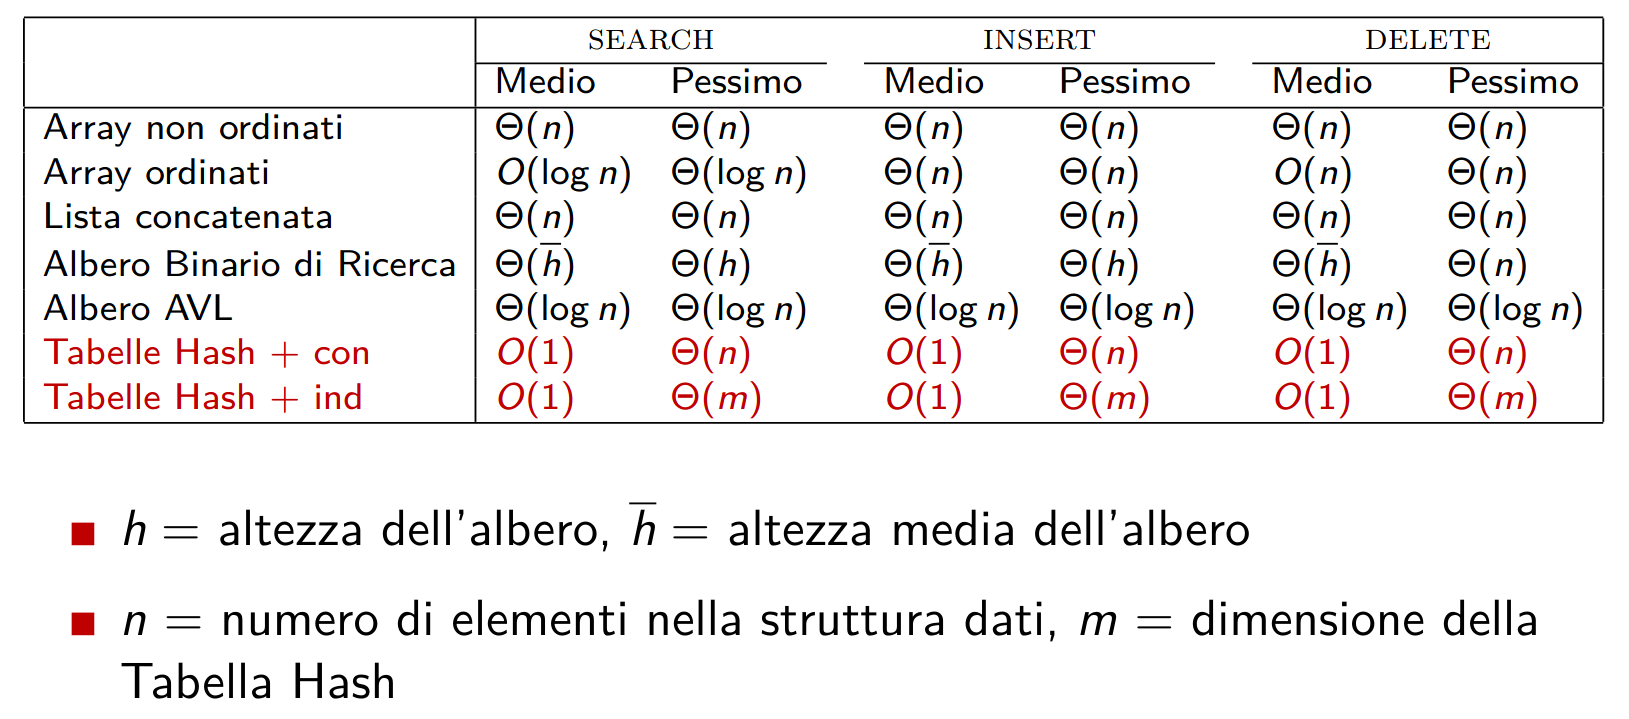
\includegraphics[width=0.75\linewidth]{Summaryhash.png}
    \caption{Riassunto costi delle strutture viste fino ad ora}
    \label{fig:summaryhash}
\end{figure}

\section{Heap binari}
L'utilizzo di questa struttura dati e' rilegata alle situazioni in cui quando si vogliono estrarre i dati essi devono essere o il minimo o il massimo dato memorizzato. Per implementare questa struttura si usano degli alberi binari \textbf{quasi perfetti} con particolari proprieta' dei nodi.
\subsection{Albero binario quasi perfetto}
Un albero binario risulta \textbf{perfetto} se ogni livello dell'albero contiene il massimo dei nodi possibili e il numero di nodi risulta essere $2^{h+1}-1$ per cui l'altezza sara' $h \approx log(N)$, con $N$ il numero di nodi. A questo punto si definisce \textbf{albero binario quasi perfetto} come un albero che e' perfetto in tutti i livelli tranne nel finale, le foglie devono essere compattate a sinistra e solo un nodo all'interno dell'albero deve avere grado minore di 2.

\subsection{Alberi heap}
\subsubsection{Max-heap} 
E' un albero binario quasi perfetto in cui ogni nodo padre contiene un valore che e' maggiore di quello del figlio, dunque la radice ha il valore massimo.
\subsubsection{Min-heap}
E' un albero binario quasi perfetto in cui ogni nodo padre contiene un valore che e' minore di quello del figlio, dunque la radice ha il valore minimo.

\subsection{Array Heap}
E' il modo piu' efficace di implementare la struttura logica ad albero: a livello logico si sta usando un albero ma in realta' a livello pratico si usa un array. Per riempire l'array bisogna fare una visita in ampiezza in modo tale da riempire l'array in ordine rispetto ai livelli dell'albero dunque il primo elemento dell'array contiene il valore piu' alto inoltre valgono le relazioni che il figlio sinistro di un elemento $i$ si trova in posizione $2i$ mentre il figlio destro si trova in posizione $2i+1$; se invece si volesse trovare il padre del nodo la sua posizone e' $\lfloor i/2\rfloor$. A questo punto si possono descrivere le varie operazioni possibili su questa struttura:
\begin{itemize}
    \item \textbf{findMax}: basta guardare il primo elemento nell'array, il costo e' $O(1)$
    \item \textbf{fixHeap}: ripristina le proprieta' di ordinamento di un max-heap rispetto ad un nodo radice. A livello implementativo quando un nodo viene sostiuito, supponendo che i suoi sotto-alberi siano a loro volta dei max heap,
    basta scambiarlo ricorsivamente con il figlio che ha il valore maggiore quando il padre non e' il massimo valore tra i figli. Nel caso pessimo il numero di scambi da effettuare e' la profondita' dell'albero ovvero $O(log(n))$.
    \item \textbf{heapify}: questa funzione si basa completaente sulla ricorsione infatti chiamato n l'indice dell'elemento che e' la radice viene chiamata ricorsivamente la funzione heapify sul sotto-albero destro e sinistro e infine chiama $fixHeap$ per sistemare l'array.
    L'equazione di ricorrenza sarebbe $T(n)=2T(n/2)+ log(n)$ ma non potendo usare il master theorem si cacola il costo con una funzione sicuramente peggiore, scambiando $log(n)$ con $\sqrt{n}$, che da come risultato un costo di $O(n)$. 
    \item \textbf{deleteMax}: rimuove l'elmento massimo e lo sostituisce con l'ultimo elemento dell'array e chiama la funzione heapfy per sistemare le proprieta' dell'albero. Il costo di questa operazione e' identico a quello dell'fixHeap ovvero $O(log(n))$.
\end{itemize}


\subsection{Heap Sort}
L'idea e' quella di costruire, a partire da un generico array, un max-heap tramite heapify poi si estrae l'elemento piu' grande come descritto prima e si va avanti cosi' fino a quando non sara' vuoto; alla fine si otterra' l'array ordinato. Il costo computazionale a questo punto risulta essere pseudolineare: $O(nlog(n))$.


\section{Coda con priorità}
E' una struttura dati che contiene delle coppie chiave-elemento, l'ordine all'interno della coda e' stabilito dalla relazione tra le varie chiavi.
Le operazioni possibili con questa struttura dati sono:
\begin{itemize}
    \item \textbf{findMin}: restituisce l'elemento associato alla chiave minima che è l'elemento nella radice. Costo costante.
    \item \textbf{insert}: inserisce una coppia nella struttura dati. Viene aggiunto l'elemento nel primo spazio disponibile e poi tramite la funzione ausiliaria muoviAlto si sistema l'elemento. Costo dell'operazione $O(log_d(n))$
    \item \textbf{delete}: rimuove un elmento dalla coda indipendentemente dalla sua chiave, supponendo un accesso diretto a tale elemento. Si sostituisce il nodo da rimuovere con l'ultima foglia e poi si usano le due funzioni ausiliarie per sistemarlo propriamente (solo una delle due entrerà in azione). Costo complessivo $O(d\ log_d(n))$.
    \item \textbf{deleteMin}: rimuove l'elemento associato alla chiave minore.
    \item \textbf{increaseKey}: rimpiazza la chiave di un elmento con una chiave maggiore, per implementarlo si cambia la chiave e poi si usa muoviBasso. Costo di $O(d \ log_d(n))$
    \item \textbf{decreaseKey}: opposto di increaseKey. In questo caso si decrementa la chiave e poi si esegue un muoviBasso per sistemare la struttura. Costo di $O(log_d(n))$
\end{itemize}

Per implementare le code con priorità ci sono due principali soluzioni ma quella che studieremo è il \textbf{D-Heap}, le implementazioni descritte sopra fanno gia' riferimento ai D-Heap.

\subsection{D-Heap}
Estendono il concetto di albero di max/min-heap binario infatti sono alberi i cui nodi al massimo hanno d figlio; nonostante ciò si basano su di essi per la loro implementazione.
In questa implementazione si usa un min-heap per cui ogni padre è il minore dei figli, in questo modo nella radice dell'albero sarà presente la chiave minima.
Anche in questo caso si ha una corrispondenza tra l'altezza dell'albero d-heap e il numero $n$ di nodi ovvero $O(log_d(n))$; come negli alberi heap binari a livello di memoria anche per gli alberi d-heap si usa un array, essendo non binari gli alberi ma $d-ari$ le relazioni tra padre e figli sono:
\begin{itemize}
    \item \textbf{Ultimo figlio}: $(i*d)+1$
    \item \textbf{Primo figlio}: $((i-1)*d)+2$
    \item \textbf{Padre del nodo}: $\lceil (i-1)/d \rceil$
\end{itemize}
Ci sono anche alcune operazioni ausiliarie alle altre procedure ovvero:
\begin{itemize}
    \item \textbf{muoviAlto}: che sposta in alto un valore che è mal posizionato, costo pari a $O(h)$.
    \item \textbf{muoviBasso}: fa il contrario di muoviAlto portando in basso l'elemento. Il costo è pari a $O(dh)$.
\end{itemize}

\subsection{Riassunto D-Heap}
\begin{figure}[H]
    \centering
    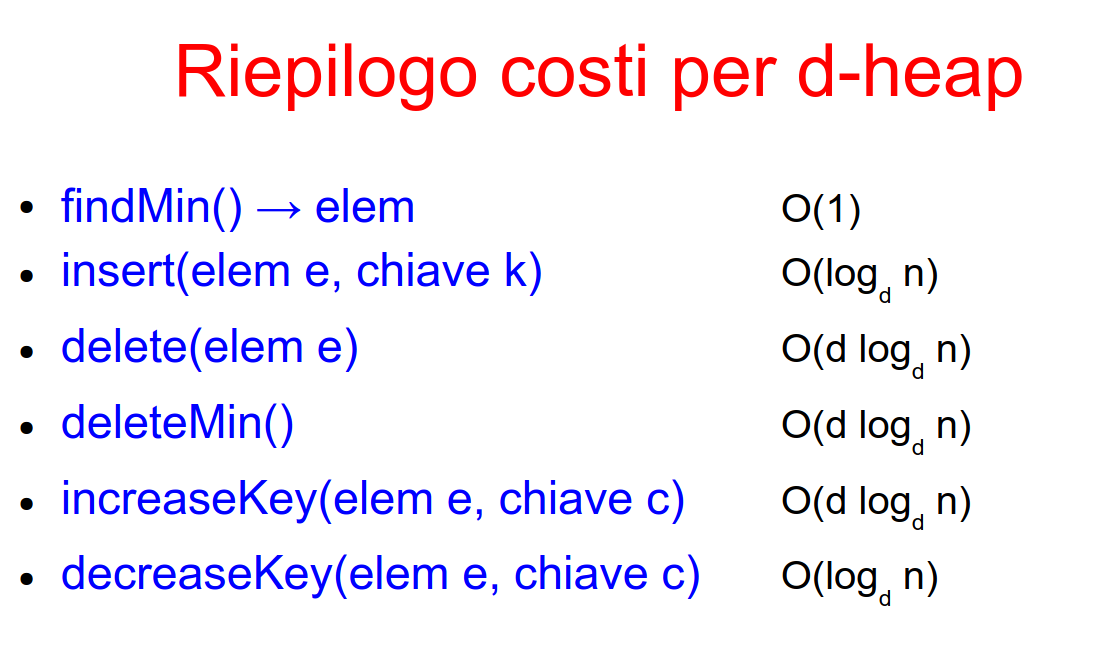
\includegraphics[width=0.75\linewidth]{Summary_d_Heap.png}
    \caption{Riassunto costi delle procedure relative ai d-heap}
    \label{fig:summarydheap}
\end{figure}


\section{Union Find}
Questa struttura dati viene impigata quando si ha la necessità di gestire insiemi disgiunti di oggetti, 
per cui le operazioni fondamentali saranno la creazione di un singoletto, unione di due insiemi e l'identificazione a quale insieme appartiene un dato elemento, piu' precisamente identificare il \textbf{rappresentante} del tale elemento.
\begin{itemize}
    \item \textbf{makeSet}: crea l'insieme singoletto con il dato elemento
    \item \textbf{find}: restituisce il rappresentante dell'insieme a cui appartiene il dato elemento
    \item \textbf{union}: unisce due insiemi di cui sono stati forniti i rappresentanti
\end{itemize}

\subsection{QuickFind}
L'implementazione della struttura dati si basa su alberi con altezza 1: ogni elemento e' una foglia e il rappresentante e' la radice (quindi il rappresentante e' un duplicato essendo sia radice che foglia).
\begin{itemize}
    \item makeSet: crea un albero con l'elemento che e' sia radice che foglia.
    \item find: dato l'elemento restituisce il proprio padre, dunque questi alberi hanno i puntatori invertiti rispetto a come si implementano di solito.
    \item union: e' la piu' dispendiosa perche' prende il secondo albero passato (la radice) e cambia tutti i puntatori dei figli facendoli puntare al nuovo padre, nel caso pessimo deve svolgere questa operazione $n-1$ volte.
\end{itemize}
\subsubsection{Euristica sul peso (union)}
Grazie a questo algoritmo si sceglie quale rappresentante mantenere, tra i due dati in input, in base a quanti figli essi hanno (basta riservare un campo specifico nel rappresentante e sommare i numeri ad ogni invocazione). Dunque nel caso pessimo si dovranno eseguire $\frac{n} {2}$ operazioni e attraverso un'analisi ammortizzata il costo risulta essere $O(log(n))$

\subsection{QuickUnion}
Questi algoritmi utilizzano alberi generali per implementare la struttura dati Union-find: 
in questo caso gli elementi possono essere anche nodi per cui il rappresentante e' il nodo che non ha padre, ovvero la radice dell'albero.
\begin{itemize}
    \item makeSet: crea un albero con l'elemento (no duplicati tra radice e foglia).
    \item find: scorre l'albero andando verso l'alto fino a quando non arriva alla radice, nel caso pessimo deve quindi scorrere tutti gli elementi.
    \item union: dati i due insiemi fa puntare il rappresentante del secondo al rappresentante del primo, per cui ha costo costante.
\end{itemize}
\subsubsection{Euristica "union by rank" (find)}
Avere alberi molto alti rende molto inefficiente l'operazione di find quindi memorizzando nelle radici il proprio rank (altezza) si puo' sistamare l'albero in modo tale che non degeneri in una lista. Grazie a questo approccio il costo scende a $O(log(n))$.

\subsection{Riassunto Union Find}
\begin{figure}[H]
    \centering
    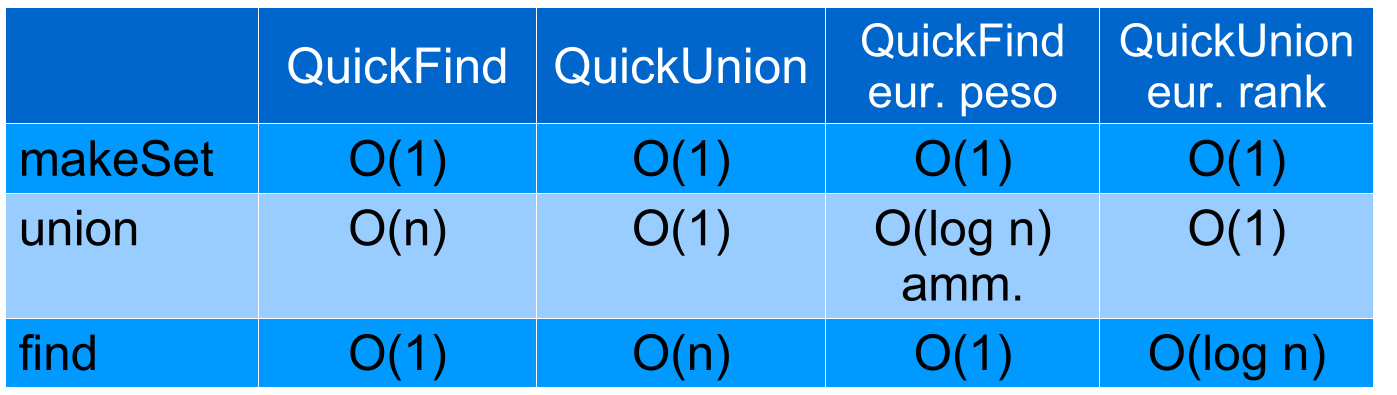
\includegraphics[width=0.75\linewidth]{Summary_Union_Find.png}
    \caption{Riassunto costi delle procedure relative alla struttura Union Find}
    \label{fig:summaryUF}
\end{figure}


\section{Tecniche algoritmiche}
\begin{itemize}
    \item \textbf{Divide-et-impera}: un problema viene diviso in sotto-problemi da risolvere ricorsivamente (top-down).
    \item \textbf{Greedy}: Ad ogni passo si fa sempre la scelta che in quel momento eà a migliore e non si ripercorrono mai le scelte fatte in precedenza.
    \item \textbf{Programmazione dinamica}: la soluzione viene costruita con un approccio bottom-up a partire da un insieme di sotto-problemi.
\end{itemize}

\subsection{Torre di Hanoi}
E' un gioco matematico in cui ci sono 3 pioli, $n$ dischi in un piolo in ordine crescente e l'obiettivo e' trasferire l'intera pila su un altro piolo.
Le regole sono che si puo' spostare un disco alla volte e che un disco deve essere impilato solo sui dischi piu' grandi di esso.
Per risolverso si usa l'approccio \textit{divide et impera}: nel caso di un solo disco lo si sposta dal primo al terzo piolo, nel caso di $n$ dischi se ne spostano $n-1$ sul secondo piolo (usando il terzo come appoggio), 
si sposta l'$n-esimo$ disco dal primo al terzo e alla fine si rispostano gli $n-1$ dischi dal secondo al terzo piolo, usano il primo come appoggio.
L'analisi del costo computazionale si puo' fare tramite l'equazione di ricorrenza $T(n) = 2T(n-1)+1$ e usando la tecnica dell'iterazione si arriva ad avere un costo totale pari a $O(2^n)$

\subsection{Problema del resto}
Dato un numero intero positivo $R$ bisgona generare qual è il minimo numero di monete che permette di raggiungere quel resto.
In questo caso l'approccio greedy e' quello che funziona meglio: ad ogni passo prendo il numero massimo di moneta piu' grande possibile e poi procedo con il taglio piu' piccolo e la rimanente parte di resto, questo sapendo che nel peggiore dei casi copriro' l'eventuale rimanenza con le monete da 1c; per cui questa soluzione funziona solo con \textbf{sistemi monetari canonici} infatti, per esempio, con monete = [4, 3, 1] e resto 6 questo approccio fornisce come soluzione {4, 1, 1} quando la soluzione ottimale sarebbe {3, 3}.



\subsection{Problema dell'imbianchino}
E' un problema simile a quello del resto: si vuole imbiancare una certa parete per cui servono $L$ litri di vernice e si vuole comprare la giusta quantità di barattoli per avere $L$ litri.
Come visto prima l'approccio greedy non e' efficace in tutte le situazioni per cui si puo' usare la tecnica \textit{divide-et-impera} che nel caso in cui i litri siano 0 ritorni 0, nel caso in cui non esistano volumi minori o uguali ritorni $\infty$.
Nel caso in cui esistano barattoli minori o uguali ai litri di vernice da comprare devo scegliere l'$i-esimo$ barattolo di vernice tale che il numero di barattoli da comperare (+1) per 
imbiancare $V_{tot}-V_{i-esimo\ barattolo}$ sia minimo.
Volendo rappresentare graficamente le operazioni attraverso un albero ci si accorge che molti risultati vengono calcolati piu' volte dunque si puo' usare la \textbf{programmazione dinamica}
per evitaredi ripetere i calcoli. In questo caso si puo' usare un array di appoggio: $SOLUZIONI[0, ..., n]$ ($con\ n = litri\ da\ comperare$) che salva la migliore soluzione per ogni $j \in [0,...,n]$ in modo da calcolre una sola volta
la soluzione ottima per ogni litro. Alla fine la soluzione al problema sara' in $SOLUZIONI[n]$.

\subsection{Problema dello zaino}
Da un insieme di oggetti $X=\{1,...,n\}$ in cui ogni $i-esimo$ oggetto ha un peso ($p[i]$), un valore ($v[i]$) e uno zaino che puo' portare un peso massimo $P$,
si vuole determinare un sott'insieme di $X$ tale che il peso degli oggetti di $X$ sia minore o uguale a $P$ e il valore di essi sia massimo.
In elenco alcune soluzioni sbagliate seguendo un approccio \textbf{greedy}:
\begin{itemize}
    \item Ad ogni passo scelgo sempre l'oggetto disponibile con valore maggiore che si può mettere nello zaino finchè non finisce lo spazio oppure nessun oggetto può essere inserito.
    \item Si calcola un valore specifico dell'oggetto (valore/peso) e si prende sempre quello piu' conveniente possibile.
\end{itemize}
Entrambe le situazioni proposte sopra non sono efficaci perchè non trovano sempre la combinazione migliore per cui è necessario un approccio che si basa sulla programmazione dinamica.
Prima di coinvolgere una struttura dati e' utile definire un sotto-problema $P(i,j)$ ovvero riempire uno zaino di capienza $j$ usando un sott'insieme dei primi $i$ oggetti;
la soluzione a questo sotto-problema ($V[i,j]$) e' il \textbf{massimo valore} ottenibile con capacita' $j$ e $i$ oggetti predibili.
A questo punto si adopera una soluzione \textbf{divide et impera}:
\begin{itemize}
\item \textbf{$V[i,0] = 0$} ovvero se non c'e' posto il valore e' nullo.
\item \textbf{$V[1,j]$} nel caso sia disponibile un solo oggetto si puo' prendere o meno a seconda del peso.
\item \textbf{$V[i,j]$:} 
        \begin{itemize}
            \item \textbf{$j < p[i] \rightarrow V[i,j] = V[i-1,j]$} ovvero se l'$i-esimo$ oggetto ha un peso troppo grande allora non va considerato l'oggetto.
            \item \textbf{$j \geq p[i] \rightarrow V[i,j] = max\{ A[i-1, j], A[i-1, j-p[i]] + v[i]\}$}   ovvero bisogna prendere il massimo valore tra il valore nel caso non prendessimo l'$i-esimo$ oggetto
                    e il valore nel caso prendessimo l'$i-esimo$ oggetto andando pero' a togliere del peso.
        \end{itemize}  
\end{itemize}
Dunque si usera' una matrice $i X j$ (numero di oggetti presi X capienza) che conterra' i risultati, la soluzione al problema sara' in $V[n,P]$ ma sara' il valore massimo trasportabile e non quali oggetti si devono prendere.
Per sapere quale sia la combinazione giusta di oggetti occorre un seconda tabella booleana che viene riempita contemporaneamente alla prima nel seguente modo:
$k[i,j] = true$ sse l'$i-esimo$ oggetto fa parte delle soluzione ottima per $P[i,j]$, in altre parole se il massimo nell'espressione di prima e' il secondo argomento.
Per stampare la soluzione si parte dall'ultima casella e si torna verso in su secondo la formula $K[i-1, j-p\_oggetto]$ solo nel caso in cui si sia trovato True se no si torna alla casella sopra.

\subsection{Esempi di utilizzo metodo Divide et Impera}
\subsubsection{Moltiplicazioni di interi di grandezza arbitraria}
La maggior limitazione delle moltiplicazione è il $max\ int$ che passato un certo limite rende errati tutti i calcoli dunque sono necessari algoritmi per moltiplicare tra di loro numeri molto grandi. 
Inizialemnte si può pensare di implementare un algoritmo basato su come si fanno le moltiplicazioni in colonna ma esso ha un costo computazionale di $O(n^2)$ per cui è necessaria una versiona più veloce, 
attraverso il metodo \textit{divide et impera} questo algoritmo può essere implementato dividento in due parti i due numeri:
\begin{center}
    $X=X_1*10^{n/2} + X_0$

    $Y=Y_1*10^{n/2} + Y_0$

    $X*Y = (X_1*10^{n/2} + X_0) (Y_1*10^{n/2} + Y_0) = (X_1*Y_1)* 10^{n} + (X_1*Y_0 + X_0 * Y_1)*10^{n/2} + X_0*Y_0$
\end{center}

Ricordando che moltiplicare per $10^n$ richiede tempo $O(n)$, l'equazione di ricorrenza $4T(n/2) + c_2n$, 
attraverso il Master Theorem si trova una complessità di $O(n^2)$ per cui non c'è alcun miglioramento rispetto a quello normale.
Per migliorare si riscrivono gli addendi in modo furbo:
\begin{itemize}
    \item $P_1 = (X_1+X_0)*(Y_1+Y_0)$
    \item $P_2 = X_1*Y_1$
    \item $P_3 = X_0*Y_0$
    \item $X*Y = P_2*10^n + (P_1-P_2-P_3)*10^{n/2}+P_3$
\end{itemize}
Quindi sono necessarie 3 moltiplicazioni che generano una lunghezza dell'output di $O(n/2)$ cifre 
quindi l'equazione di ricorrenza di prima cambia in $3T(n/2)+c_2*n$ arrivando a $O(n^{log_2(3)}) \approx O(n^{1.59})$

\subsubsection{Sottovettore non vuoto di valore massimo}
Il problema prevede di trovare un sottovettore ad un array dato (quindi elementi contigui) la cui somma sia massima. 
Il metodo \textit{brute force} che calcola il valore di ogni combinazione ha un costo di $O(n^3)$ che puoò essere migliorato mantenendo in una variabile il valore della sommatoria precedente  portando ad un costo $O(n^2)$. 
Con il metodo \textit{divide et impera} l'idea è quella di trovare un pivot e calcolare il sottovettore massimo a destra del pivot, a sinistra del pivot e il massimo valore a cavallo con il pivot.
Per calcolare il massimo a destra e a sinistra basta una chiamata ricorsiva mentre per il sotto-array a cavallo servono due cicli che scorrono a destra e a sinistra del pivot. 
Per trovare il valore massimo si usano due variabili $somma$ e $massimo$: la prima viene incrementata ad ogni elemento del valore dello stesso mentre la seconda viene cambiata tutte le volte che la prima raggiunge un nuovo massimo. 
L'equazione di ricorrenza è dunque $T(n) = 2T(n/2)+n$ con un costo totale di $O(n\ logn(n))$.

\subsection{Esempi di utilizzo metodo Greedy}
\subsubsection{Problema di scheduling}
Dati dei "job" da eseguire con un certo tempo di esecuzione l'obiettivo è trovare l'ordine (scheduling) che dia il \textbf{minimo tempo di attesa medio} ovvero ogni quanto un nuovo job è iniziato. 
Per questo motivo l'ordine migliore è quello che mette in ordine dal più corto al più lungo dunque l'approccio greedy è il migliore dunque si implementa un algoritmo che mandi in esecuzione iljob con minor tempo richiesto ancora da fare.

\subsubsection{Problema della compressione (codifica di Huffman)}
Il problema che si vuole risolvere e' quello della rappresentazione di delle sequenze di caratteri: data una sequenza vogliamo un codifica, tramite tecnica detta \textbf{codifica dei caratteri}, che minimizzi la lunghezza e che sia possibile decifrare in modo \textbf{sequenziale}.
La soluzione migliore è una \textbf{codifica a lunghezza variabile} che si basa sulla percentuale di apparizione del carattere:
 a caratteri che appaiono più spesso associo una codifica più corta e man mano aumento la lunghezza della sequenza codificante.
Questa operazione deve mantenere un \textbf{codice a prefisso} cioe' nessun codice non può essere il prefisso di un altro codice in modo tale che appena si individua un carattere si sa che può essere solo quello. 
Per rappresentare il codice di codifica/decodifica si puo' usare un albero binario in cui ogni figlio di sinistra rappresenta uno zero e quello di destra un uno, nelle foglie si troveranno i caratteri.
Per creare quest'albero si usa l'\textbf{algoritmo di Huffman}:
\begin{enumerate}
    \item Costruzione di una lista \textbf{ordinata} in cui ogni nodo e' una coppia $(carattere, frequenza\ di\ apparizione)$
    \item Rimuovere i due nodi con frequenza minore e collegarli ad un padre che abbia la frequenza con somma delle frequenze dei nodi figli.
    \item Aggiungere il nodo padre alla lista mettendolo in ordine.
    \item Ripetere fino a quando non rimane un solo nodo. 
\end{enumerate}
L'albero creato con queste caratteristiche ha la stessa caratteristica dei figli di quello descritto sopra perche' il codice e' strettamente correlato al singolo file.


\subsection{Esempi di utilizzo di programmazione dinamica}
E' una tecnica iterativa che affronta i problemi con un approccio \textit{bottom-up} e che è molto vantaggiosa quando si tratta di risolvere sottoproblemi ripetuti, comporta sempre l'appoggio ad una struttura dati ausiliaria.
\subsubsection{Numero di Fibonacci, tecnica della Memorization}
Questa tecnica usa una struttura \textit{cache} (ovvero un array) che memorizza i valori intermedi che sono già stati calcolati 
evitando cosi' di ripetere calcoli gia' eseguiti. 
Un ulteriore modifca per rendere l'algoritmo piu' efficiente a livello di memoria e' quella di usare una array di dimensione 3 per salvare $fib(n-2), fib(n-1), fib(n)$.

\subsubsection{Sottovettore di valore masismo}
E' il problema gia' affrontato con la tecnica \textit{divide et impera}, per risolverlo con la programmazione dinamica 
si ultilizza un vettore soluzione $S[i,...,n]$ che viene riempito secondo la formula $max\{V[i], V[i] + S[i-1]\}$, ovvero chiedendosi
se la soluzione per il sotto-vettore $V[0,...,i-1]$ sommata a $V[i]$ e' migliore o peggiore di $V[i]$. 
Per trovare \textbf{quale} sia tale sotto-vettore basta trovare il massimo di $S$ nella posizione $i$ (esso sara' lo stesso indice dell'ultimo elemento di $V$ del sotto-vettore massimo)
e andare a ritroso in $V$ fin quando la somma degli elementi $V[i]+...+V[x]$ non e' ugule al valore di $S[i]$. 


\subsubsection{Seam Carving}
Il problema e' quello di voler ridimensionare un'immagine tagliando solo delle cuciture di pixel adiacenti removibili,
 i "pixel removibili" sono quelli con valore assegnatoli, tramite algoritmi non studiati, minore. 
Essendo l'immagine iniziale una matrice anche la struttura dati di appoggio sara' la medesima, delle medesime dimensioni.
Per quanto riguarda l'algoritmo in se' si tratta di stabilire, partendo dall'ultima riga, qual e' il valore del percorso piu' "basso" che parte dalla cima: 
ricorsivamente si va a calcolare il valore minimo per le 3 caselle adiacenti sopra. 
Una volta riempita la matrice di appoggio con gli opportuni valori, per trovare la cucitura da eliminare basta trovare il minimo valore presente nell'ultima riga e da risalire fino alla cima selezionando le caselle che nella matrice d'appoggio hanno valore minore tramite un approccio greedy.


\subsubsection{Distanza di Levenshtein}
E' il problema che affrontano i controllori ortografici quando suggeriscono parole simili come correzioni a quelle digitate;
la loro somiglianza tra due stringhe di caratteri si basa sul concetto di \textbf{edit distance} ovvero il numero di operazioni necessarie per trasformare una stringa T in una stringa S. 
Le uniche trasformazioni ammesse sono: \begin{itemize}
    \item Lasciare immutato il carattere   $\rightarrow$ costo 0
    \item Cancellare un carattere $\rightarrow$ costo 1
    \item Inserire un carattere $\rightarrow$ costo 1
    \item Sostituire un carattere con uno differente $\rightarrow$ costo 1
\end{itemize}
Ovviamente la conversione viene operata carattere per carattere sulla stringa T.
Per definizione la \textbf{distanza di Levenshtein} tra $S[1 .. n]$ e $T[1 .. m]$ e' il costo minimo (riferito a quelli esplicitati prima) tra tutte le sequenze di \textit{operazioni di editing} che trasformano S in T.
Per determinare la distanza di Levenshtein definisamo il sotto-problema $P(i,j)$: determinare il minor numero di operazioni per trasformare $S[1,...,i]$ in $T[1,...,j]$.
Per calcolare le soluzioni $L[i,j]$:
\begin{verbatim}
    if (i==0 \lor j==0) // nel caso ci sia una sequenza nulla bisogna 
                        //trasformarla in quella non nulla
        L[i,j] = max{i,j};
    else if (S[i] == T[j])
        L[i,j] = min{L[i-1,j]+1,L[i,j-1]+1,L[i-1,j-1]}; //devo prendere il minimo di operazioni tra 
                                                        //trasformare S[1,...,i-1] in T[1,..,j] ed 
                                                        //eliminare l'ultimo carattere, fare lo stesso
                                                        // ma a sequenze invertite oppure trasformare 
                                                        //S[1,...,i-1] in T[1,...,j-1] e lasciare 
                                                        //l'ultimo carattere invariato
    else
        L[i,j] = min{L[i-1,j]+1,L[i,j-1]+1,L[i-1,j-1]+1}; //devo prendere il minimo di operazioni tra 
                                                        //trasformare S[1,...,i-1] in T[1,..,j] ed 
                                                        //eliminare l'ultimo carattere, fare lo stesso
                                                        // ma a sequenze invertite oppure trasformare 
                                                        //S[1,...,i-1] in T[1,...,j-1] e cambiare solo 
                                                        //l'ultimo carattere
\end{verbatim}

Per memorizzare le soluzioni si utilizzera' una matrice $L=nXm$ e la distanza di Levenshtein si trovera' in $L[n,m]$


\section{Grafi}
Sono strutture dati che permettono di memorizzare quanto i diversi elementi si interfacciano tra di loro, 
i problemi che affronteremo sui grafi sono la \textbf{visita} (in ampiezza e in profondità), \textbf{alberi di copertura minimi} e \textbf{cammini minimi} (in caso di singola sorgente e fra tutte le coppie).
Ci sono due definizioni di grafo che distinguono i due tipi:
\begin{itemize}
    \item \textbf{Grafo orientato}: è una coppia di insiemi, il primo è quello dei vertici e il secondo e' quello delle relazioni tra i vertici. 
    Viene definito \textbf{cappio} un nodo in relazione con se stesso.
    \item \textbf{Grafo non orientato}: gli archi (ovvero le relazioni tra elementi) sono non ordinate (quindi non c'è una direzione) e i cappi non sono ammessi.
\end{itemize}
Ci sono alcune definizioni che sono utili per questa struttura tipo l'\textbf{incidenza} che, in un grafo orientato, indica che un arco e' in relazione tra due vertici; 
se due nodi sono \textbf{adiacenti} significa che c'è una relazione tra i due (ovvero ci si può arrivare).
Le operazioni di base che il grafo deve supportare sono:
\begin{multicols}{2}
\begin{itemize}
    \item NumVertici $\to$ int
    \item NumArchi $\to$ int
    \item grado (vertice) $\to$ int ($n.collegmaneti$)
    \item archiIncidenti $\to$ (arco, ..., arco)
    \item estremi (arco) $\to$ (vertice, vertice)
    \item sonoAdiacenti (vertice, vertice) $\to$ bool
    \item aggiungiVertice 
    \item aggiungiArco
    \item rimuoviVertice
    \item rimuoviArco
\end{itemize}
\end{multicols}

\subsection{Implementazione grafo non orientato, matrice di adiacenza}
Si usa una matrice con tutti gli elementi sia nelle righe che nelle colonne e si mette 1 se due elementi sono collegati 0 se non lo sono. Quella che risulta è una matrice simmetrica con diagonale tutta 0 per l'assenza cappi.
Lo spazio necessario è $\Theta(|V|^2)$. I costi delle operazioni sono:
\begin{multicols}{2}
\begin{itemize}
    \item grado $\rightarrow$  $\Theta(n)$
    \item archiIncidenti $\rightarrow$ $\Theta(n)$
    \item sonoAdiacenti  $\rightarrow$ $\Theta(1)$
    \item aggiungiVertice $\rightarrow$ $\Theta(n^2)$
    \item aggiungiArco $\rightarrow$ $\Theta(1)$
    \item rimuoviVertice $\rightarrow$ $\Theta(n^2)$
    \item rimuoviArco $\rightarrow$ $\Theta(1)$
\end{itemize}
\end{multicols}

\subsection{Implementazione grafo non orientato, lista di adiacenza}
L'idea è quella di avere un array degli elementi che sono inizi di liste che contengono gli elementi a cui sono adiacenti, lo spazio di memoria è $\Theta(|V|+|E|)$ con V vertici e E le relazioni.
Di seguito i costi delle operazioni ricordando che $\delta(x)$ e' il grado del nodo x e $m$ il numero di archi:
\begin{multicols}{2}
\begin{itemize}
    \item grado $\rightarrow$  $\Theta(\delta(v))$
    \item archiIncidenti $\rightarrow$ $\Theta(\delta(v))$
    \item sonoAdiacenti $\rightarrow$ $\Theta(min\{\delta(x),\delta(y)\})$
    \item aggiungiVertice $\rightarrow$ $\Theta(1)$
    \item aggiungiArco $\rightarrow$ $\Theta(1)$
    \item rimuoviVertice $\rightarrow$ $\Theta(m)$
    \item rimuoviArco $\rightarrow$ $\Theta(\delta(x)+\delta(y))$, arco = $\{x,y\}$
\end{itemize}
\end{multicols}
\subsection{Implementazione grafo orientato, matrice di adiacenza}
L'implementazione e' molto simile a quella per il grafo non orientato ma la matrice non e' piu' simmetrica perche' l'ordine 
di relazione conta in questo caso. Nello specifico il vertice di partenza e' nelle righe e quello di arrivo nelle colonne.

\subsection{Implementazione grafo orientato, lista di adiacenza}
Anche questa implementazione e' molto simile a quella per il grafo non orientato, la differenza e' che l'elemento dell'array indica 
il nodo di partenza e la lista contiene quelli a cui si puo' arrivare ma non vale il contrario.


\subsection{Alcune definizioni}
\begin{enumerate}
    \item \textbf{Grafi pesati}: sono grafi in cui ogni arco ha un peso/costo, per determinare il costo si utilizza un'opportuna funzione che, per comodità, restituisce $\infty$ quando non c'è una relazione tra i due elementi. 
    Nel caso di un implementazione con matrice di adiacenza quando c'e' un arco tra due vertici al posto di 1 si mette il costo, al posto di 0 si mette $\infty$.
    Per la lista lista di adiacenza invece l'arco ha un campo che ne indica il peso.
    \item \textbf{Grado}: dato un grafo non orientato il grado di un vertice è il numero di archi del dato vertice.
    Nel caso di grafo orientato c'è la distinzione in \textbf{grado entrante} e \textbf{grado uscente} ovvero il numero di archi in arrivo e in uscita.
    \item \textbf{Cammino}: percorso che collega due vertici, se esiste si dice che $w$ è raggiungibile da $v$ tramite il cammino $w$.
    La lunghezza del cammino e' pari al numero di vertici attraversati -1 oppure al numero di archi attraversati; 
    un cammino e' \textbf{semplice} se i vertici compaiono una volta.
    Nel caso di grafi orientati il cammino prende in considerazione l'orientamento dei collegamenti.
    \item \textbf{Grafi connessi}: nel caso del grafo non orientato esso è connesso se esiste un cammino che da ogni vertice arriva ad ogni altro vertice.
    Nel caso del grafo orientato esso è \textbf{fortemente connesso} se esiste un cammino da ogni vertice ad ogni altro vertice mentre si dice \textbf{debolmente connesso} se l'equivalente non orientato del grafo orientato è connsesso.
    \item \textbf{Ciclo}: cammino che parte da un elemento e attraversa un grafo ritornandoci. Nel caso di grafo orientato bisogna fare almeno 1 passo mentre in quelli non orientati almeno 3 passi.
    Un \textbf{ciclo semplice} è un cammino che non ritorno su nessun nodo già attraversato, mentre il \textbf{ciclo complesso} ha dei nodi ripetuti nel cammino.
    \item \textbf{Grafi aciclici}: un grafo non orientato è aciclico se è senza cicli semplici mentre quello orientato lo è solo se non ci sono cicli.
    \item \textbf{Grafo completo}: un Grafo non orientato è completo se ha un arco per ogni possibile vertice, per calcolare il numero di archi necessari a ciò si può usare la formula: $\frac{|V|*(|V|-1)} {2}$
    \item \textbf{Albero}: un \textbf{albero libero} è un grafo non orientato connesso e aciclico, mentre se chiamiamo uno dei vertice radice otteniamo un \textbf{albero radicato}
\end{enumerate}


\subsection{Algoritmi di visita dei grafi}
Dato un grafo ed un vertice (\textbf{sorgente}) l'obiettivo è visitare ogni possibile vertice del grafo raggiungibile dalla sorgente una sola volta.
\subsubsection{Visita in ampiezza (BFS)}
Visita i nodi espandendo la frontiera tra nodi scoperti e nodi da scoprire. Alla fine dell'esecuzione ha creato un albero radicato in $s$ (il nodo di partenza) che contiene tutti i nodi che si posso raggiungere da esso.
Durante l'esecuzione un nodo puo' essere: \textbf{inesplorato} ovvero non ancora incontrato, \textbf{aperto} ovvero quando viene incontrato la prima volta oppure \textbf{chiuso} ovvero il vertice e' stato esplorato completamente.
Per quanto riguarda l'implementazione essa si basa su il campo $mark$ di ogni nodo che inizialmente setta in tutti i nodi a $false$ e poi grazie ad una coda apre un nodo, mette in coda tutti i nodi non aperti raggiungibili da quello analizzato, chiude il nodo e continua con il successivo nodo in coda.
Per quanto riguarda la creazione dell'albero ad ogni nodo adiacente che viene aperto si riempie il campo $parent$ con il nodo che si sta analizzando. Alla fine viene ritornato l'albero.
Per quanto riguarda la complessità computazionale nel caso di \textit{liste di adiacenza} e' $O(n+m)$ mentre nel caso della \textit{matrice di adiacenza} e' di $O(n^2)$, con $n$ numero di vertici e $m$ numero di archi.
Questo tipo di visita e' utile per capire quale sia il cammino piu' breve tra due nodi nel caso ci sia una BFS partita dal nodo di inizio: 
si crea l'albero e poi, partendo dal nodo finale, tramite una funzione ricorsiva che a ritroso arriva fino al nodo di inizio si può stampare il cammino più corto.


\begin{verbatim}
    Tree BFS (Graph G, Vertex s){
        for (Vertex v : Graph.getVertexes)
            v.mark = false;
        
        Tree T = s;
        s.mark = true;
        Queue Q = new Queue;
        Q.enqueue(s);
        while (!Q.isEmpty()){
            Vertex vert = Q.dequeue;
            for (Vertex adiacent : vert.GetAdiacents){
                if (adiacent.mark == false) {
                    adiacent.mark = true;
                    adiacent.parent = vert;
                    adiacent.distance = vert.distance + 1;
                    Q.enqueue(adiacent);
                }
            }
        }
        return T;
    }
\end{verbatim}


\subsubsection{Visita in profondità (DFS)}
Visita i nodi andando il più possibile lontano dalla sorgente e a differenza del BFS arriva a tutti i nodi del grafo, non solo quelli collegati ad un nodo. Per questo motivo la funzione crea un foresta ovvero un insieme di alberi.
L'algoritmo e' ricorsivo e per ogni nodo riempie due parametri: un \textit{discorvery time} ovvero il momento in cui e' stato scoperto e un \textit{finish time} ovvero quando termina la visita del nodo. 
La visita funziona che parte dal nodo iniziale al momento 1 poi passa ad un altro nodo fino a quando non si arriva ad un nodo che non ha piu' nodi non ancora scoperti disponibili.
A quel punto tale nodo viene chiuso l'esecuzione torna sul nodo precedente e se ha altri nodi adiacenti inesplorati salta a loro se no anche esso viene chiuso e così via fino a quando tutti i nodi sono chiusi; 
questo viene controllato da un ciclo while che si assicura che tutti i nodi del grafo siano stati considerati per cui anche nodi non connesi al nodo iniziale vengono considerati.
Gli alberi vengono creati come prima ma essendo che si guardano tutti i nodi in casi di nodi scollegati o cappi vengono restituiti piu' alberi.
Per quanto riguarda la complessità essa rimane invariata rispetto al BFS perche' i passaggi di inizializzazione dei campi necessari allo svolgimento sono quelli piu' dispendiosi.
Grazie ai campi \textbf{discorvery time} e \textbf{finish time}  di due nodi si possono avere diverse informazioni in base alla relazione tra gli intervalli:
\begin{itemize}
    \item $[u.dt,\ u.ft]$ e $[v.dt,\ v.ft]$ sono \textbf{disgiunti} allora u e v non sono discendenti.
    \item $[u.dt,\ u.ft]$ e' contenuto in $[v.dt,\ v.ft]$ allora u e' discendente di v.
    \item $[u.dt,\ u.ft]$ contiene $[v.dt,\ v.ft]$ allora v e' discendente di u.
\end{itemize}
Mentre nel caso di grafi orientati, nel caso di un arco non incluso nella foresta:
\begin{itemize}
    \item $v.dt < u.dt \land u.ft < v.ft$ allora l'arco $(u,v)$ e' all'\textbf{indietro}. 
    \item $u.dt < v.dt \land v.ft < u.ft$ allora l'arco $(u,v)$ e' in \textbf{avanti}.
    \item $v.ft < u.dt$ allora l'arco $(u,v)$ e' \textbf{di attraversamento a sinistra}.
\end{itemize}
Per quanto riguarda le applicazioni questa visita rende particolarmente facile \textbf{Verificare DAG (Direct Acyclic Graph)} ovvero verificare che non ci siano archi all'indietro e fare l'\textbf{ordinamento topologico} nella sottocategoria dei DAG.
L'ordinamento topologico è interessante perchè può essere interpretato come dipendenze logiche tra eventi tipo catena di montaggio. L'algoritmo si basa appunto su un iniziale DFS e ritorno una lista che viene fatta mettendo in ordine decrescente i finish time di ogni nodo, in modo pratico si fa una head-push ogni volta che un nodo viene chiuso.

\begin{verbatim}
    global int time = 0;

    Tree DFS (Graph G){
        for (Vertex v : Graph.getVertexes){
            v.mark = false;
            v.parent = null;
        }
        
        Tree T;
        for (Vertex vert : G.getVertexes){
            if (vert.mark == false)
                T = DFS_search(vert);
        }
        return T;
    }

    Tree DFS_search (Vertex vert){
        vert.mark = true;
        vert.dt = time;
        time++;
        for (Vertex v : vert.GetAdiacents){
            if (v.mark == false){
                v.parent = vert;
                DFS_search(v);
            }
        }
        time ++;
        vert.ft = time;
        return vert; //as a tree
    }

\end{verbatim}

 
\subsection{Componenti connesse (grafi non orientati)}
Due vertici $u$ e $v$ di un grafo sono \textbf{connessi} quando e' possibile raggiungere $v$ partendo da $u$, questa definizione induce un possibile partizionamento del grafo in insiemi di nodi connessi tra di loro.\
Per risolvere questo problema basta etichettare inizialmente tutti i nodi con un valore di "non visitato" poi, per ogni nodo non ancora visitato, si chiama una funzione ricorsiva che etichetta con un valore (che per ogni insieme differente deve cambiare) il nodo, riempie il campo $parent$ dei nodi come nelle altre visite e si richiama ricorsivamente sui nodi connessi.

\subsection{Componenti fortemente connesse (grafi orientati)}
Si esegue un iniziale partizionamento del grafo di tutti i vertici fortemente connessi tra loro, per fare questo basta calcolare $D(x)$ ovvero tutti i discendenti del nodo $x$ e $A(x)$ ovvero l'insieme di tutti i nodi da cui si può raggiungere $x$.
Per calcolare $D(x)$ basta fare una visita qualunque per calcolare $A(x)$ basta invertire la direzione degli archi e fare una nuova ricerca partendo sempre da $x$.
A questo punto per avere il partizionamento cercato basta calcolare $D(x) \cap A(x)$.
Per risolvere il problema di partizionare l'intero grafo tra i suoi elementi fortementi connessi tra di loro basta iterare l'algoritmo per ogni nodo e trovare l'intersezione tra tutti i nodi.
La complessità computazionale è di $O(nm+n^2)$ per cui in realtà esistono algoritmi più efficienti.


\subsection{Minimum Spanning Tree}
Il problema è quello di voler determinare come connettere gli elementi di un grafo tra di loro usando collegamenti meno pesanti possibili; il grafo non è orientato ma è connesso e pesato. 
E' come se si volesse collegare con la fibra ottica un paese usando meno cavo possibile.
Per trovare la combinazione giusta bisogna trovare l'albero di copertura minore possibile, per \textbf{albero di copertura} si intende un sottografo di un grafo non orientato e connesso che contiene tutti i nodi del grafo, anch'esso è pesato ma come collegamenti ha un sotto insieme di quelli di partenza.
Per trovare l'\textbf{albero di copertura di peso minimo} bisgna trovare l'albero che minimizza il peso complessivo. 
Precisazione importante è quella che il problema non sempre ha una soluzione univoca e che per collegare $n$ nodi è necessario fare almeno $n-1$ passi. 
Inoltre, un arco è definito \textbf{sicuro} se aggiungendolo ad un MST l'unione rimane un MST quindi nella soluzione si devono prediligere questi archi.
Il \textbf{metodo generico} per risolvere il problema è quello di creare un albero e unirlo sempre con archi sicuri.


\subsubsection{Regole del ciclo e del taglio}
Un \textbf{taglio} di un grafo non orientato è una partizione del grafo in due sottinsiemi disgiunti e un \textbf{arco leggero} è l'arco che che costa meno e che collega i due insiemi disgiunti dal taglio; 
un arco \textbf{attraversa il taglio} se dato l'arco ${u, v}$ allora $u \in S \land v \in V-S$ con $V$ il grafo iniziale e $V - S$ il sottoinsieme post taglio.
La \textbf{regola del taglio} vuole che scelto un taglio nel grafo che non "spezza" archi già considerati come ottimi e si può prendere come ottimo quello di costo minore.
La \textbf{regola del ciclo} vuole che dato un ciclo senza archi già individuati come pessimi possiamo considerare pessimo l'arco con peso peggiore.
Applicando queste regole si puoò individuare il MST però bisogna capire come e quando applicare queste tecniche.

\subsubsection{Algoritmo di Kruskal}
Analizza gli archi in costo crescente e utilizza un approccio greedy che si basa sulle union find: se i due nodi del collegamento appartengono gia' allo stesso insieme allora esso e' un arco da scartare (si tratta di un ciclo) mentre se i due nodi sono disgiunti allora e' un ponte tra le due porzioni di taglio per cui e' il percorso ottimale.
In tutto questo per determinare l'MST ogni volta che si fa una union tra due insieme anche i nodi vengono uniti nell'albero finale
Il costo totale è $\Theta(m\ log(n))$.


\begin{verbatim}
    Tree Kruskal (Graph G) {
        PriorityQueue Q = new PriorityQueue;
        UnionFind S = new UnionFind;
        for (Edge edge : G.getEdges())
            Q.insert(edge, w(Edge));
        
        for (Vertex V : g.getVertexes()){
            S.makeSet(V);
            V.parent = null;
        }

        while (!Q.isEmpty()){
            Edge e = Q.find();
            Q.deleteMin();
            Vertex So = e.getSource():
            Vertex D = e.getDest();
            if (S.find(So) != S.find(D))
                D.parent = So;
        }
        
        return T; //Supposing T is the root of the tree.
    }
\end{verbatim}


\subsubsection{Algoritmo di Prim}
Questo algoritmo parte da un nodo e taglia i suoi cammini, procede sempre e solo con la regola del taglio ed 'espande' sempre il taglio tenendo da una parte i nodi già nell'albero (ovvero quelli esplorati) e dall'altra del taglio quelli ancora da inserire.
Per implementare questo algoritmo si usano le code con priorità: partendo dal primo nodo si inseriscono nella coda con priorità coppie $(nodo\ di\ arrivo, distanza)$ possibili (ovvero i collegamenti dal nodo in analisi) e iterativamente questo processo viene compiuto per ogni nodo secondo l'ordine nella lista con priorita'.
Per generare l'albero ogni nodo diventa il padre dei nodi che sblocca nodi o di cui riduce il cammino minimo.
A questo punto si capisce perche' nell'implementazione della coda con priorita' e' necessario prevedere il caso in cui un elemento gia' inserito sia reinserito ma con un peso differente: nel caso si sia trovata una strada piu' efficiente per un nodo esso dovra' cambiare di posizione nella coda. 
La complessità di questo algoritmo è di $\Theta(m\ log(n))$.

\begin{verbatim}
    Tree Prim (Graph G, Vertex a) {
        Tree T = a;
        PriorityQueue Q = new PriorityQueue;
        Q.enqueue(a,0);

        for (Vertex v : G.getVertexes()){
            v.mark = false;
            v.parent = mull;
            v.distance = infty;
            }
        
        while (!Q.isEmpty()){
            Vertex vert = Q.find();
            Q.deleteMin();
            if (vert.mark == false) {
                vert.mark = true;
                for (Edge e : vert.getOutEdges()){
                    if (e.getDest.mark == false){
                        Q.enqueue(e.getdest,w(e))
                        e.getDest.distance = vert.distance + w(e);
                        e.getDest.parent = vert;
                    } else if (e.getDest.distance > w(e) + vert.distance){
                        Q.decareseKey(e.getDest, w(e));
                        e.getDest.distance = vert.distance + w(e);
                        e.getDest.parent = vert;
                    }
                }
            }
    
        }
        return T;
    }
\end{verbatim}





\subsection{Camminimi minimi}
Considerando un grafo orientato e pesato si vuole trovare il cammino di costo minimo che collega due nodi dati in input. Ci sono diverse formulazioni del problema oltre a quella appena fornita, per esempio il \textit{single surce shortest path} che dato un solo punto deve restituire tutti i cammini minimi da esso agli altri oppure l'\textit{All-pairs shortest path} ovvero determinare il minimo cammino tra tutte le coppie di punti.
Ci sono dei casi in cui  non si può trovare un cammino minimo, principalmente solo due: quando i due punti non sono raggiungibili (tipo alcuni nodi di grafi orientati) oppure cammini con costo negativo all'interno di un ciclo che complessivamente ha un costo negativo perchè basta continuare a girare nel ciclo abbassando il costo. 
Ci sono alcune cose tecniche da sapere a riguardo di questo problema, per esempio se due nodi sono collegati allora esiste sempre un cammino semplice (senza cicli) si costo minimo.
Un'altra proprietà del cammino ottimale è quella di essere anche il cammino ottimale per collegare il punto di inizio con qualsiasi altro nodo intermedio a quello finale.
Inoltre si possono costruire \textbf{Alberi di costo minimo} che contengono il cammino minimo dal nodo di partenza a qualsiasi altro nodo. 
Ci sono anche alcune utili \textbf{proprietà della distanza tra vertici} tra cui:
\begin{itemize}
    \item $d_{vv} = 0 \   \forall v$
    \item $d_{xy} = min_{(z,y) \in E} (d_{xz}+w(z,y))$ ovvero se esite un cammino da $x$ a $y$ allora esiste almeno un vertice $z$ che è l'ultimo arco del camminimo minimo prima di $y$.
    Questa proprietà può suggerire un approccio divide et impera tramite una chiamata ricorsiva ma questo aprroccio in realtà non funziona.
    \item $d_{xy} = \infty$
\end {itemize}

\subsubsection{Algoritmo di Bellman Ford}
Questo algoritmo risolve il problema nella forma \textit{single surce shortest path}: data la sorgente $s$ mantiene una stima per eccesso $D_{sv} \geq d_{sv}$ del cammino minimo ad ogni nodo $v$, al termine dell'esecuzione del problema le stime saranno precise per cui $D_{sv} = d_{sv}$ sse non ci sono cicli di costo negativo.
Inizialmente pone $D_{ss} = 0, \   d_{sv} = \infty \ \forall s \not= v$, successivamente esegue dei \textit{rilassamenti} che migliorano le approssimazioni. 
Questi rilassamenti sono piuttosto intuitivi: se c'è un cammino tra un nodo intermedio tra $s$ e $v$ chiamato $D_{su}$ che sommato al cammino tra $u$ e $v$ risulta minore di $D_{sv}$ allora si sostituisce il valore della somma essendo un cammino minimo.
Per eseguire un ciclo di rilassamento bisgna anallizzare tutti gli archi del grafo vedendo se permettono un effettivo rilassamento.
A questo punto tocca capire quante iterazioni di rilassamenti devono essere fatte per arrivare ad una convergenza sicura, la risposta è che dopo $k$ iterazioni si è trovato il cammino minimo che attraversa al massimo $k$ archi.
Per cui essendoci al massimo $n-1$ archi in un grafo allora alla $n-1$ iterazione avremo coperto tutti i cammini possibili e trovato dunque il minimo, il costo computazionale è $O(nm)$.
In realtà una possibile modifica che lo rende più efficiente è terminare non sempre a $n-1$ ierazioni ma quando non si effettuano più rilassamenti, un'altra modifica è controllare se ci sono cicli negativi: basta, una volta finito il rilassamento, controllare se è possibile eseguirne un altro e in caso affermativo c'è un ciclo di costo negativo.
Il costo di questo algoritmo e' $O(nm)$

\begin{verbatim}

    //L'algoritmo e' implementato in modo tale che restituisca un albero, volendo si puo'
    //creare un array pred[1,...,n] che per ogni vertice v e il suo predecessore u
    //memorizza nell'array la relazione: pred[v] = u; 


    Tree Bellman-Ford (Graph G, Vertex a) {
        Tree T = a;
        for (Vertex v : G.getVertexes){
            v.distance = infty;
            v.parent = null;
        }
        a.distance = 0;
        bool mod = true;
        for (int i = 0; int < G.NumVertici && mod; i++){
            mod = false;
            for (Edge e : G.getEdges()){
                if (e.getDest.distance > e.getSource.distance + w(e)){
                    e.getDest.distance = e.getSource.distance + w(e);
                    e.getDest.parent = e.getSource;
                    mod = true;
                }
            }
        }
        mod = false;

        for (Edge e : G.getEdges()){
                if (e.getDest.distance > e.getSource.distance + w(e))
                    mod = true;
            }

        if (!mod)
            return T;
        else
            print "C'e' almeno un ciclo negativo";
    }
\end{verbatim}






\subsubsection{Algoritmo di Dijkstra}
Anche questo algoritmo è necesario a risolvere il \textit{single surce shortes path} che però è più efficiente di quello di Belman-Ford ma non funziona in caso di cammini negativi.
Il lemma su cui si basa questo algoritmo è che dato il grafo senza cammini negativi e un albero di cammini minimi dalla radice alle foglie allora il cammino minimo tra una foglia e un nodo non appartenente all'albero è proprio quello dalla foglia al nodo.
L'algoritmo viene implementato tramite una coda con priorita' che resituisce sempre il nodo con distanza minima disponibile, per ogni nodo aggiorna, quando e' possibile, il valore della distanza dalla sorgente di tutti i nodi a lui adiacenti, li mette nella coda e li connette ad esso nell'albero di costo minimo.
Il costo computazionale di questo algoritmo e' $O(mlog(n))$.

\begin{verbatim}
    Vertex [] Dijksta (Graph G, Vertex a) {
        Vertex pred [1,..., G.NumVertici()];
        PriorityQueue Q;
        for (Vertex v : G.getVertexes())
            v.distance = infty;
        a.distance = 0;
        pred[a] = a;
        Q.enqueue(a,0);
        while(!Q.isEmpty()){
            Vertex v = Q.findMin();
            Q.deleteMin();
            for (Edge e : v.getOutEdges()){
                if (e.getDest().distance == infty){
                    e.getDest().distance = v.distance + w(e);
                    pred[e.getDest()] = v;
                    Q.enqueue(e.getDest(), e.getDest().distance);
                } else if (e.getDest().distance > v.distance + w(e)) {
                    e.getDest().distance = v.distance + w(e)
                    pred[e.getDest()] = v;
                    Q.decareseKey(e.getDest(), e.getDest().distance);
                }
            }
        }
        return pred;
    }
\end{verbatim}



\subsubsection{Algoritmo di Floyd e Warshall}
Questo algoritmo risolve il problema dell'\textit{all-pairs shortest paths}, si basa sulla programmazione dinamica: iterativamente calcola $D_{xy}^k$ ovvero il cammino tra $x$ e $y$ usando $k$ nodi con $k=1,...,n$; 
alla fine dell' esecuzione la soluzione sara' proprio $D_{xy}^n$. Per rappresentare le soluzioni intermedie si utilizza una matrice di dimensioni del numero di nodi.
I casi base del calcolo sono semplici perche' $D_{xy}^0$ e' $0$ se $x=y$, $w(x,y)$ se sono collegati mentre $\infty$ se non sono collegati.
Per calcolare tutti gli altri sotto-problemi si usa la formula $D_{xy}^k = min\{D_{xy}^k-1, D_{xk}^k-1 + D_{ky}^k-1\}$, ovvero ci si chiede se, andando da $x$ a $y$, e' piu' conveniente andarci direttamente oppure andare da $x$ a $k$ e poi da $k$ a $y$.
Si inizializza una matrice 3 dimensionale che ha lati: n, n, n+1 le righe sono la partenza, le colonne l'arrivo e la profondita' e' la pesantezza del cammino da $x \rightarrow y$; 
la prima facciata e' $D_{xy}^0$ con x,y che sono i due possibili vertici (cosi' si analizzano tutte le combinazioni).
 A questo punto con un ciclo diverso si itera la formula precedente per ogni $n + 1$ faccia del cubo e su ogni cella della singola faccia.
L'ultima facciata pero' non ci offre anche un modo di trovare un cammino per cui e' necessatrio utilizzare una matrice d'appoggio che tutte le volte che si trova un cammino migliore memorizza, nella matrice d'appoggio, il nodo successivo a quello analizzato.
A questo la tabella d'appoggio per ogni coppia $(partenza, arrivo)$ contiene il passo successivo da fare e cosi' si puo' trovare il cammino minimo.
Dunque la complessita' computazionale e' $O(n^3)$, si puo' effettuare una piccola ottimizzazione a livello di memoria: al posto di usare un cubo si puo' usare una tabella normale che cambia ad ogni iterazione ma il valore $k$ e' ancora necessario per la quantita' di iterazioni.
Inoltre si possono anche individuare i cicli negativi nel grafo: a iterazione finita basta controllare se la distanza tra un vertice e se stesso e' inferiore a 0.

\begin{verbatim}
    Vertex [] [] Floyd_Warshall (Graph G) {
        int n = G.NumVertici();
        Vertex M [n] [n];
        Vertex pred [n][n]
        for (int i = 0; i < n; i++){
            for (int j = 0; j < n; j++){
                if (i == j)
                    M[i][j] = 0;
                else if (G.getEdge(i,j) != null)
                    M[i][j] = w(G.getEdge(i,j));
                else
                    M[i][j] = infty;
            }
        }
        for (int k = 0; k < n; k++){
           for (int i = 0; i < n; i++){
                for (int j = 0; j < n; j++){
                    if (M[i][j] > M[i][k] + M[k][j]){
                        M[i][j] = M[i][k] + M[k][j]
                        pred[i][j] = pred [i] [k];
                    }
                }
            } 
        }
        for (int i = 0; i < n; i++) {
            if ( D[x,x] < 0 ) then
                error “Il grafo contiene cicli negativi”
            else
                return pred;
        }
    }
\end{verbatim}



\section{Tabella riassuntiva di tutti i costi visti}

\begin{center}
\begin{tabular}{||c | c c c||} 
 \hline
 Algoritmo & Costo ottimo & Costo medio & Costo pessimo \\ [0.5ex] 
 \hline\hline
 SelectioSort & $\Theta(n^2)$ & $\Theta(n^2)$ & $\Theta(n^2)$ \\ 
 \hline
 InsertionSort & $\Theta(n)$ & $\Theta(n^2)$ & $\Theta(n^2)$ \\
 \hline
 MergeSort & $\Theta(n\ log(n))$ & $\Theta(n\ log(n))$ & $\Theta(n\ log(n))$ \\
 \hline
 QuickSort & $\Theta(n\ log(n))$ & $\Theta(n\ log(n))$ & $\Theta(n^2)$ \\
 \hline
 CountingSort & $\Theta(n + k)$ & $\Theta(n + k)$ & $\Theta(n + k)$ \\  
 \hline
 RadixSort & $\Theta(d(n + k))$ & $\Theta(d(n + k))$ & $\Theta(d(n + k))$ \\ [0.5ex] 
 \hline
 findMin & & & $O(1)$\\
 \hline
 insert & & & $O(log_d(n))$\\
 \hline
 delete & & & $O(d\ log_d(n))$\\
 \hline
 deleteMin & & & $O(log_d(n))$\\
 \hline
 increaseKey & & & $O(d\ log_d(n))$\\
 \hline
 decareseKey & & & $O(log_d(n))$\\
 \hline
\end{tabular}
\end{center}
Legenda:
\begin{itemize}
    \item n = numero di elementi da ordinare
    \item d = numero massimo di cifre in una chiave
    \item k = ampiezza range di valori chiave
\end {itemize}
\begin{figure}[H]
    \centering
    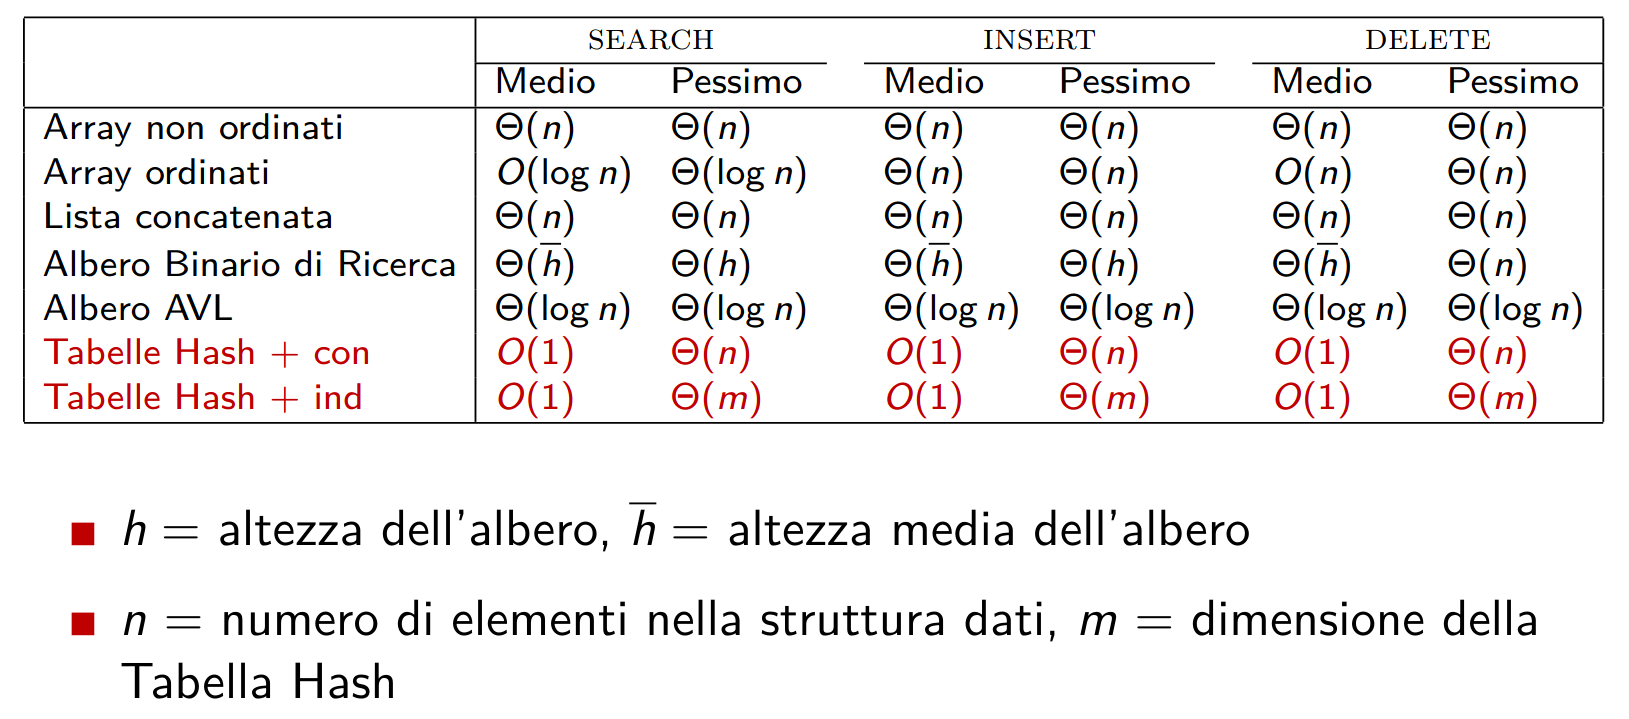
\includegraphics[width=0.75\linewidth]{Summaryhash.png}
    \caption{Riassunto costi delle operazioni su un dizionario implmentato con le diverse strutture viste}
    \label{fig:summaryhash}
\end{figure}


\begin{figure}[H]
    \centering
    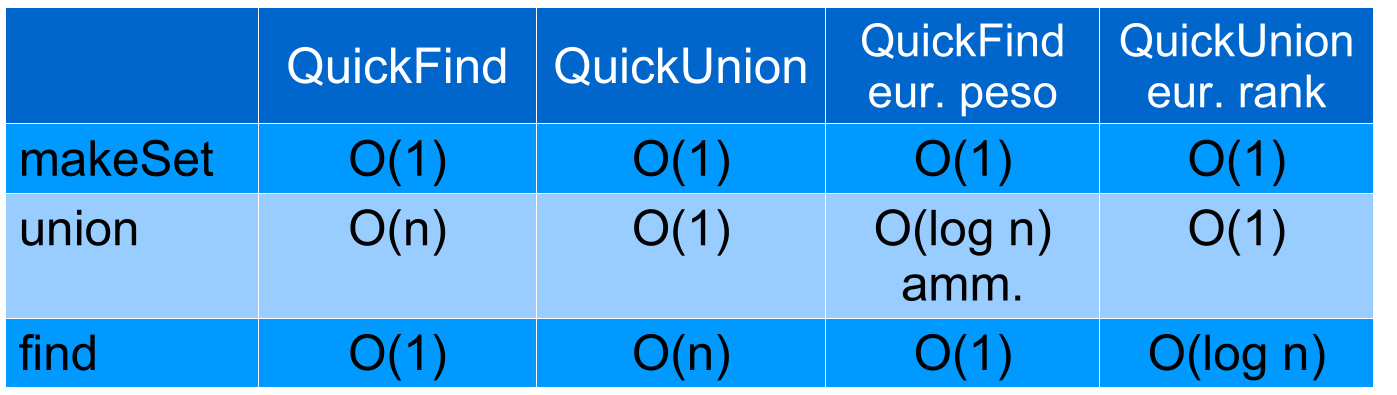
\includegraphics[width=0.75\linewidth]{Summary_Union_Find.png}
    \caption{Riassunto costi delle procedure relative alla struttura Union Find}
    \label{fig:summaryUF}
\end{figure}

\begin{center}
\begin{tabular}{||c | c c||} 
 \hline
 Algoritmo & Matrice di Adiacenza & Lista di Adiacenza \\ [0.5ex] 
 \hline\hline
 BFS & $O(n^2)$ & $O(n + m)$ \\ 
 \hline
 DFS & $O(n^2)$ & $O(n + m)$ \\ 
 \hline
 Kruskal &  & $O(m\ log(n))$ \\ 
 \hline
 Prim &  & $O(m\ log(n))$  \\ 
 \hline
 Bellman Ford &  & $O(nm)$ \\ 
 \hline
 Dijksta &  & $O(m\ log(n))$ \\ 
 \hline
 Floyd Warshall &  & $O(n^3)$ \\ 
 \hline
\end{tabular}
\end{center}


\end{document}